\chapter{Learning zeros of Fokker-Planck operators}
\section{Introduction}\label{sec-intro--steady-fp}Many real world problems can be modelled as the response of nonlinear systems to random excitations and such systems have been a topic of interest for a long time. Stochastic differential equations (SDE) provide the natural language for describing these systems. Although SDEs have their origins in the study of Brownian motion by Einstein and Smoluchowski, it was Itô who first developed the mathematical theory. Since then SDEs have extensively appeared in physics \cite{lelievre2016partial}, \cite{strauss2017hitch},      \cite{ivanov1980method}, biology \cite{allen2010introduction}, mathematical finance \cite{delong2013backward}, \cite{karoui1997non}, and many other fields \cite{oksendal2003stochastic}, \cite{gardiner2009stochastic}. 
The probability density associated with an Itô SDE evolves in time according to a Fokker-Planck equation (FPE) or Kolmogorov forward equation. A stationary FPE (SFPE) can be solved analytically when the corresponding Itô SDE has a drift term that can be represented as the gradient of some potential \cite{risken1996fokker}. 
But the same is not true when the drift is not of the aforementioned form. And the time-dependent FPE does not admit a closed form solution in general even when the drift is integrable. Since the solution of an FPE is a probability density, the boundary condition is replaced by an integral condition which is extremely hard to implement in dimensions larger than 2.

In recent times deep learning has been successfully used to solve high-dimensional PDEs \cite{sirignano2018dgm}, \cite{han2018solving}, \cite{raissi2019physics}. Although universal approximation theorems \cite{pinkus1999approximation}, \cite{lu2020universal}, \cite{de2021approximation}, \cite{kovachki2021universal} guarantee existence of neural networks that approximate the true solution well, due to the non-convex nature of loss functions one can not guarantee convergence of neural networks to the true solution during training in many instances \cite{krishnapriyan2021characterizing}, \cite{basir2022investigating}.
Moreover, these methods are almost always used for PDEs with simple boundary conditions not containing integral terms which makes applying them for FPEs challenging. But even though deep learning solutions to PDEs is fraught with challenges, it is a worthwhile paradigm to work in while dealing with high-dimensional PDEs for the following reasons. 
Most deep learning methods are mesh-free \cite{blechschmidt2021three} and can deal with the curse of dimensionality much better than classical methods \cite{cioica2022deep}. Moreover, some of them focus on computing pointwise solutions to PDEs \cite{han2018solving} which albeit non-standard, might be the only practical and efficient approach in high dimensions. 

The goal of this paper is to devise a reliable, mesh-free deep learning algorithm to find non-trivial zeros of high-dimensional Fokker-Planck operators. In a sequel we will devise a method for solving high-dimensional time-dependent FPEs using these zeros. Although our algorithm is capable of handling any non-solenoidal drift function, as examples we focus on problems where the underlying ODE system possesses a global attractor. These systems are often used to make simple models in the earth sciences and provide ideal test cases for non-linear filtering algorithms \cite{carrassi2022data}. We solve 2,3,4,6,8 and 10 dimensional problems with our method. We compare our method with Monte Carlo for $d=2$, investigate how the loss function and the distance from the true solution are related to each other and explore how our method scales with dimension.



\section{Problem statement}
\label{sec-prob--steady-fp}In this work, we are interested in problems of the following form.
\begin{equation}
\begin{aligned}
    &\underset{u\in X}\arginf f(u)\\
    &\subto g(u)=0 
\end{aligned}   \label{eq:con-opt--var-ml}
\end{equation}
where $f :X\to\mathbb R$ and $g: X\to W$ and $X, W$ are real Hilbert spaces. $X$, in particular, is an infinite dimensional Hilbert space whereas $W$ can be either finite or infinite dimensional. This ensures that problem~\eqref{eq:con-opt--var-ml} is indeed an infinite-dimensional optimization problem. This setup allows us to encompass a fairly large class of problems with one or multiple constraints or even unconstrained problems if we set $g$ to be the zero function. 
% But we can always reformulate the constraint $g(u)=0$ as 
% \begin{align}
%     \|g(u)\|_W = 0
% \end{align}
% where $\langle\cdot\rangle_W$ and $\|\cdot\|_W$ are the inner product and norm on $W$ respectively. Therefore, it suffices to assume $g:X\to\mathbb R$.
To better familiarize ourselves with this setup let us first look at a few examples.
\subsection{The minimal surface problem} During the later half of the eighteenth century Lagrange in his correspondence of with Euler delineated the foundations of calculus of variations and derived the famous Euler-Lagrange formula \cite{goldstine2012history}. One of the problems he considered during this time, asks to find the surface of least area stretched across a given contour. Although Lagrange did not find any solutions other than the plane, Euler and Jean Baptiste Meusnier later showed that helicoid and catenoid are also valid solutions to the minimal surface problem \cite{meusnier1785memoire}. Since then the theory of minimal surfaces has seen multiple revivals with Schwarz's solution to the Björling problem \cite{darboux1896leccons}, the discovery of Costa's surface \cite{costa1984example} and has even found its way into mathematical physics through topics like positive energy theorem \cite{schoen1979proof}. The rich theory behind minimal surfaces allows them to be expressed in many different ways \cite{colding2011course}. Here we will work with a definition that closely resembles Lagrange's original formulation. Rather than describing the minimal surface problem in its full generality, we describe the specific problem we will solve below. We define $X$ to be an appropriate Sobolev space, $f$ to be an area functional and $g$ to be the boundary condition.
\begin{equation}
\begin{aligned}
    &\Omega=(0,1 )\times(-2\pi, 2\pi),\;X=W^{1, 2}(\Omega;\mathbb R),\; W=W^{1,2}((-2\pi,2\pi);\mathbb R)\\
    &f(u)=\int_{-2\pi}^{2\pi}\int_0^1\sqrt{\left[1+\left(\frac{\partial u}{\partial r}\right)^2\right]r^2+\left(\frac{\partial u}{\partial\theta}\right)^2}\;dr\,d\theta\\
&g(u): \theta \mapsto u(1, \theta) - \theta\label{eq:ms--var-ml}
\end{aligned}    
\end{equation}
Our question thus becomes, what is the surface of minimal area given it has a unit helix as its boundary? And the solution $u^*$ gives us the minimal surface $(r, \theta, u^*(r,\theta))$. 

\subsection{Geodesics on a surface}  Johann Bernoulli was interested in several problems in calculus of variations and investigated both curves of shortest length and time between two points \cite{struik1961lectures}, \cite{goldstine2012history}. The former type of curves are known as geodesics while the latter are known as brachistochrones. After having found the solution to the brachistochrone problem Bernoulli had challenged his contemporaries to come up with their own solutions (a practice that was not uncommon in the era) to which Newton (anonymously), Jacob Bernoulli, Leibniz and de L'Hôpital had responded with their own solutions. The aftermath of this challenge would eventually lead to the infamous calculus controversy between Leibniz and Newton \cite{palomo2021new}, \cite{goldstine2012history}. Even though the brachistochrone problem is one of the oldest problems to be posed in calculus of variations with a rich history of mathematical rivalry associated with it, the geodesic problem would go on to outpace it in terms of importance with the development of differential geometry. Eventually geodesics would become an essential part in our understanding of motion under gravity with the advent of general relativity \cite{weinberg1972gravitation}. Here we look at the simple problem of finding the shortest path on unit a sphere given two points $(1, \theta_0, \phi_0), (1, \theta_1, \phi_1)$ (in spherical polar coordinates) on it by setting,
\begin{equation}
\begin{aligned}
    &\Omega=[\theta_0, \theta_1],\;X=W^{1, 2}(\Omega; [0, 2\pi)),\; W=\mathbb R\\
    &f(u) = \int_{\theta_0}^{\theta_1}\sqrt{1+\left(\sin\theta \frac{du}{d\theta}\right)^2}\;\,d\theta\\
    & g(u) = \sqrt{(u(\theta_0)-\phi_0)^2 + (u(\theta_1)-\phi_1)^2}\label{eq:gs--var-ml}
\end{aligned}
\end{equation}
If $u^*$ is the solution then $(1,\theta, u^*(\theta))$ gives us a parametrization for the geodesic curve.
\subsection{Grad-Shafranov equation} Grad-Shafranov equation is an elliptic partial differential equation describing the poloidal flux under ideal magnetohydrodynamics for a 2D plasma \cite{smithaaxisymmetric}.  Modelling the plasma equilibrium is an important aspect of designing magnetic confinement devices like tokamaks in the field of nuclear fusion. Although originally used for axis-symmetric tokamaks, the Grad-Shafranov equation has been analyzed for non-axis symmetric magnetohydrodynamic equilibrium as well \cite{burby2020generalized}. In 1968 Solov'ev derived a family of analytic solutions for the Grad-Shafranov equation under the assumption that there is distributed toroidal
current filling all space \cite{xu2019vacuum} and since then these Solev'ev solutions have become an import benchmarking tool for plasma equilibrium codes \cite{johnson1979numerical}. Below we describe the Grad-Shafranov equation, this specific version can also be found in \cite{xu2019vacuum}. 
\begin{equation}
\begin{aligned}
    &\frac{\partial^2 u}{\partial z^2}+r\frac{\partial}{\partial r}\left(\frac{1}{r}\frac{\partial u}{\partial r}\right) =ar^2 + bR^2,\qquad (r,z)\in\Omega= [0.9R, 1.1R]\times[-0.1R, 0.1R]\\
    & u(r, z) = \frac{1}{2}(b+c_0)R^2z^2+c_0R\zeta z^2+\frac{1}{2}(a-c_0)R^2\zeta^2, \qquad (r, z)\in{\partial\Omega}\\
    &\text{\rm where }\zeta =\frac{r^2-R^2}{2R}, R=1.0,\, a = 1.2,\,b=-1.0,\, c_0=1.1
\end{aligned}
\end{equation}
In order to cast this problem into the format of \eqref{eq:con-opt--var-ml}, we set
\begin{equation}
\begin{aligned}
    &X = W^{1,2}(\Omega;\mathbb R),\;W=W^{1,2}(\partial\Omega; \mathbb R)\\
    &f(u) = \int_{-0.1R}^{0.1R}\int_{0.9R}^{1.1R}\left(\frac{\partial^2 u}{\partial z^2}+r\frac{\partial}{\partial r}\left(\frac{1}{r}\frac{\partial u}{\partial r}\right) -ar^2 - bR^2\right)^2\,dr\,dz\\
    &g(u): (r,z)\mapsto \frac{1}{2}(b+c_0)R^2z^2+c_0R\zeta z^2+\frac{1}{2}(a-c_0)R^2\zeta^2 - u(r, z)
\end{aligned}\label{eq:GS--var-ml}
\end{equation}
\subsection{Beltrami fields} Beltrami fields are special vector fields that are eigenfunctions of the curl operator. They play an important role in fluid dynamics as steady solutions to the Euler equation \cite{aris2012vectors}. In this problem we ask, given Beltrami boundary data, what is the magnetic field of least energy in a 3D volume? Gauss's law \cite{jackson1999classical} dictates that we have to take the nondivergence of magnetic fields into account which can be done in multiple ways while formulating our question, either as a part of the Hilbert space $X$ (since divergence is a linear operator) or as an addition to the boundary condition $g$. Here we choose to impose Gauss's law as a part of the Hilbert space $X$.
\begin{equation}
    \begin{aligned}
&\Omega = \left[-\frac{1}{2}, \frac{1}{2}\right]^3,\; X=\overline{\{u\in W^{1,2}(\Omega; \mathbb R^3):\nabla\cdot u=0\}},\;W=W^{1,2}(\partial\Omega;\mathbb R^3)\\
    &f(u) = \frac{1}{2}\int_{-\frac{1}{2}}^{\frac{1}{2}}\int_{-\frac{1}{2}}^{\frac{1}{2}}\int_{-\frac{1}{2}}^{\frac{1}{2}}|u(x, y, z)|^2\,dx\,dy\,dz\\
    & g(u): (x, y, z)\mapsto u(x, y, z) - \begin{bmatrix}
\sin(z) + \cos(y) \\
\sin(x) + \cos(z) \\
\sin(y) + \cos(x) \\
\end{bmatrix}
    \end{aligned}
\end{equation}
Unlike the other problems stated here, this problem is \textit{manufactured} and has no direct practical applications but nevertheless serves as an interesting toy problem.

\section{Previous works}\label{sec-prev-work--steady-fp}An extensive amount of work has been done on the topic of numerically solving Fokker-Planck equations. A large amount of these works are based on traditional PDE solving techniques like finite difference \cite{berezin1987conservative}, \cite{whitney1970finite}, \cite{sepehrian2015numerical} and finite element \cite{naprstek2014finite}, \cite{masud2005application} methods. For a comparison of these traditional methods the reader can look at this comparative study \cite{pichler2013numerical} by Pitcher et al where the methods have been applied to 2 and 3 dimensional examples. 


In recent times efforts have been made to devise methods that are applicable in dimensions higher than 3. Tensor decomposition methods  \cite{Hackbusch2005HierarchicalKT}, \cite{kolda2009tensor} are an important toolkit while dealing with high-dimensional problems and they are proving to be useful in designing numerical solvers for PDEs \cite{ballani2013projection}, \cite{kressner2010krylov}.  For stationary Fokker-Planck equations Sun and Kumar proposed a tensor decomposition and Chebyshev spectral differentiation based method \cite{sun2014numerical} in 2014. In this method drift functions are approximated with a sum of functions that are separable in spatial variables, an well-established paradigm for solving PDEs. The differential operator for the stationary FPE is then discretized and finally a least sqaures problem is solved to find the final solution. The normalization is enforced via addition of a  penalty term in the optimization problem. The high-dimensional integral for the normalization constraint in this method is replaced with  products of one dimensional integrals and therefore becomes computable.   

In 2017 Chen and Majda proposed another hybrid method \cite{chen2018efficient} that utilizes both kernel and sample based density approximation to solve FPEs that originate from a specific type of SDE referred to as a conditional Gaussian model,
\begin{equation}
\begin{aligned}
    d\mathbf{u_I} = [A_0(t, \mathbf{u_I}) + A_1(t, \mathbf{u_I})\mathbf{u_{II}}]\,dt + \Sigma_I(t, \mathbf{u_I})\,dW_I(t)\\
    d\mathbf{u_{II}} = [a_0(t, \mathbf{u_I}) + a_1(t, \mathbf{u_I})\mathbf{u_{II}}]\,dt + \Sigma_{II}(t, \mathbf{u_I})\,dW_{II}(t)\label{eq:conditional-Gaussian-SDE}
\end{aligned}
\end{equation}
This special structure of the SDE allows one to approximate $p(\mathbf{u_{II}}(t))$ as a Gaussian mixture with parameters that satisfy auxiliary SDEs. $p(\mathbf{u_I}(t))$ is approximated with a non-parametric kernel based method. Finally the joint distribution $p(\mathbf{u_I}(t), \mathbf{u_{II}}(t))$ is computed with a hybrid expression. Using this method Chen and Majda computed the solution to a 6 dimensional conceptual model for turbulence. Note that, among our examples only L63 falls under this special  structure.

In recent years machine learning has also been applied to solve SFPEs. In 2019 Xu et al solved  2 and 3 dimensional stationary FPEs with deep learning \cite{xu2020solving}. Their method enforced normalization via a penalty term in the loss function that represented a Monte-Carlo estimate of the solution integrated over $\mathbb R^d$. Although simple and effective in lower dimensions, this normalization strategy loses effectiveness in higher dimensions. Zhai et al \cite{zhai2022deep} have proposed a combination of deep learning and Monte-Carlo method to solve stationary FPEs. The normalization constraint here is replaced with a regularizing term in the loss function which tries to make sure the final solution is close to a pre-computed Monte-Carlo solution. This strategy is more effective than having to approximate high-dimensional integrals and the authors successfully apply their method on Chen and Majda's 6 dimensional example.








\section{Overview of deep learning}
\label{sec-learning--steady-fp}
In this section we describe the general process of \textit{learning} a solution to a partial differential equation. The strategy described here will be an integral part of the final algorithm. In what follows next, we see how to see solve a generic PDE independent of time on a bounded domain with a Dirichlet boundary condition in a \textit{physics-informed} manner.  The interested reader can see \cite{raissi2019physics}, \cite{blechschmidt2021three}, \cite{sirignano2018dgm} for more discussions. In the next few subsections we keep simplifying our PDE problem until it finally becomes solvable on a computer.

\subsection{From PDE to optimization problem} In the context of machine learning, \textit{learning} refers to solving an optimization problem. So to solve our PDE with deep learning we first transform it into an optimization problem. Suppose our 2nd order PDE looks like, 
\begin{equation}
\begin{aligned}
    &\mathcal Lf(\mathbf x) = 0,\quad \mathbf x\in\Omega \,, \\
    &f(\mathbf x) = g(\mathbf x),\quad \mathbf x\in\partial\Omega \,,
\end{aligned}\label{eq:generic-pde}
\end{equation}
and just like before we are interested in finding a solution in $W^{1,2}(\Omega)\cap C^2(\Omega)$. Instead of trying to solve \eqref{eq:generic-pde} a popular strategy is to try to solve the following problem (see for example \cite{sirignano2018dgm}),
\begin{align}
    \min_{f\in W^{1,2}(\Omega)\cap C^2(\Omega)}\left[\int_\Omega (\mathcal L f)^2 + \int_{\partial\Omega}(f-g)^2\right]\label{eq:generic-pde-opt}
\end{align}
The choice of function space ensures one-to-one correspondence between the solutions of the PDE and the optimization problem.

\subsection{From infinite-dimensional search space to finite-dimensional search space}\label{ssec-infinite-to-finite} To solve a problem on a machine with finite resources we need to finitize the infinite aspects of the problem. We then solve the finitized problem which preferably approximates the original problem well to get an approximate solution to the orginal problem. For \eqref{eq:generic-pde-opt} our search space $W^{1,2}(\Omega)\cap  C^2(\Omega)$ is infinite dimensional which we need to replace with a finite dimensional search space.
In order to finitize the dimension of the search space we appeal to universal approximation theorems that say neural networks of even the simplest architectures are dense in continuous functions, see for example theorem 3.2 in \cite{kidger2020universal} or proposition 3.7 in \cite{pinkus1999approximation}. Universal approximation theorems typically allow networks to have either arbitrary depth or arbitrary width in order to achieve density \cite{pinkus1999approximation}, \cite{de2021approximation}. But the sets of neural networks with arbitrary depth or width are still infinite dimensional and therefore are infeasible to work with. In practice, we fix an architecture $\mathcal A$ with a fixed number of layers and trainable parameters and work with the following set instead.
\begin{align}
    S_{\mathcal A}\stackrel{\rm def}{=}\{n^{\mathcal A}_\theta: \theta\in \mathbb R^C\}\label{eq:search-space-net}
\end{align}
Here $n^{\mathcal A}_\theta$ is a network with architecture $\mathcal A$ with trainable parameters $\theta$ and $C$ is the total number of trainable parameters or the size of $\theta$. Since $C$ is fixed, $S_{\mathcal A}$ has a one-to-one correspondence with $\mathbb R^C$ and therefore is finite-dimensional. Even though we lose the density argument while working with $\theta$ of fixed size, in recent times it has been shown that sets like $S_\mathcal A$ are not closed in $W^{1, 2}(\Omega)$ and can, in principle, be used as good function approximators, see \cite{mahan2021nonclosedness} for a detailed discussion. In the following discussion we suppress the architecture and use $n^{\mathcal A}_\theta$ and $n_\theta$ interchangably for notational convenience. After restricting our search space to \eqref{eq:search-space-net},  \eqref{eq:generic-pde-opt} becomes,
\begin{align}
    \min_{\theta\in\mathbb R^C}\left[\int_{\Omega} (\mathcal L n_\theta)^2 + \int_{\partial\Omega}(n_\theta-g)^2\right]\label{eq:generic-pde-opt-theta}
\end{align}

\subsection{From integrals to sums} 
The domain $\Omega$ in our examples will often be of such a dimension that will make computing the integrals in \eqref{eq:generic-pde-opt-theta} extremely challenging. To deal with this we will replace the integrals in \eqref{eq:generic-pde-opt-theta} with Monte-Carlo sums as follows,

\begin{align}
    \min_{\theta\in\mathbb R^C}\left[\frac{1}{N}\sum_{j=1}^N (\mathcal L n_\theta(\mathbf x_j))^2 + \frac{1}{M}\sum_{j=1}^M(n_\theta(\mathbf y_j)-g(\mathbf y_j))^2\right]\label{eq:generic-opt-final}
\end{align}
where $\{\mathbf x_j\}_{j=1}^N$, $\{\mathbf y_j\}_{j=1}^M$ are uniform samples from $\Omega$ and $\partial \Omega$ respectively.

\subsection{Finding the optimal parameters}\label{ssec-finding-theta}
We simply perform gradient descent with respect to $\theta$ to find the optimal network for the problem \eqref{eq:generic-opt-final}. The Monte-Carlo sample sizes should be dictated by the hardware available to the practitioner.  In our experiments $N=M=1000$. In higher dimensions these choices are not enough to capture the original integrals entirely in one go. In that case \eqref{eq:generic-opt-final} can interpreted as trying to find a network that satisfies the original problem \eqref{eq:generic-pde} at the specified points $\{\mathbf x_j\}_{j=1}^N, \{\mathbf y_j\}_{j=1}^M$, which we can refer to as \textit{collocation points}. But in our experiments we try to the learn the solution on the entire domain as thoroughly as possible and so we resample the domain every few training iterations. So even though we are limited in sample-size by our hardware, we can shift the burden on space or memory to time or number of training iterations and adequately sample the entire domain. This principle of space-time trade-off is ubiquitous in machine learning \cite{buduma2022fundamentals} and comes in many different flavours like mini-batch gradient descent, stochastic gradient descent etc. Even though in this paradigm we are not training our network with typical input-output pairs, our method can be thought of as a variant of the mini-batch gradient descent.

\subsection{Why deep learning}
Deep learning in this context refers to learning an approximate solution to \eqref{eq:generic-pde} with the outlined method with an architecture $\mathcal A$ that is \textit{deep} or has many hidden layers. Deep networks are more efficient as approximators than shallow networks in the sense that they require far fewer number of trainable parameters to achieve the same level of approximation, for a discussion see section 5 of \cite{holstermann2023expressive}. Now that we have described the general procedure of \textit{deep learning} a solution to a PDE, we will pause briefly to point out some benefits and demerits of this approach. Deep learning has, like any other method some disadvantages. 
\begin{itemize}
    \item Deep learning is slower and less accurate for lower dimensional problems for which standard solvers exist and have been in consistent development for many decades. 
    \item Most modern GPUs are optimized for computation with single-precision or float32 numbers. This is efficient for rendering polygons or other image processing tasks which are the primary reasons GPUs were invented \cite{peddie2023history} but float32 might be not accurate enough for scientific computing. Although not ideal, this problem will most likely disappear in the future.
    \item The objective or \textit{loss} function used in a typical problem might not be convex and hence difficult to deal with \cite{krishnapriyan2021characterizing}, \cite{basir2022investigating}. 
\end{itemize}
But even with these disadvantages, the benefits of deep learning make it a worthwhile tool for solving PDEs.
\begin{itemize}
    \item Since we don't need to deal with meshes or grids in this method, we can mitigate the curse of dimensionality in memory. It will be clear from our experiments that the size of the network or $C$ does not need to grow exponentially with the dimensions. This method lets one compute the solution at collocation points but if one wants to compute the solution over the entire domain, one needs to sample the entire domain thoroughly which can be done in a sequential manner without requiring more memory as discussed in~\ref{ssec-finding-theta}.
    \item All derivatives are computed with automatic differentiation and therefore are accurate upto floating point errors. Moreover, finite difference schemes do not satisfy some fundamental properties of differentiation e.g. the product rule \cite{ranocha2019mimetic}. With automatic differentiation one does not have to deal with such problems. 
    \item If one computes the solution over the entire domain, the solution is obtained in a functional form which can be differentiated, integrated etc.
    \item Other than a method for sampling no modifications are required for accommodating different domains. 
\end{itemize}


\section{The algorithm}
\label{sec-algo--steady-fp}In this section we outline the algorithm for learning zeros of FPOs. But before that we go through the primary challenges and ways to mitigate them.

\subsection{Unboundedness of the problem domain}\label{ssec-unbounded-domain--steady-fp} We can try the same procedure as outlined in section~\ref{sec-learning--steady-fp} to find a non-trivial zero of $\mathcal L$. But computationally we can only deal with a bounded domain. Hence we focus on a compact domain which contains most of the mass of the solution to \eqref{eq:SFPE-0--steady-fp}. We refer to this domain as the \textit{domain of interest} $\Omega_I$ in the following discussion. \textcolor{magenta}{We note that the support of non-trivial zeros of $\mathcal L$ will usually be unbounded and of course we do not know the domain that may contain most of the mass. Thus the choice of $\Omega_I$ needs to be informed by some a priori knowledge of the solution, which in the examples we discuss is related to some attracting set of the deterministic system associated to the drift term $\mu$, i.e., the first term in~\eqref{eq-sde--steady-fp}. We do not need a precise knowledge of such an attracting set. But the smaller the domain $\Omega_I$, the more efficient will be the proposed method which requires uniform samples from $\Omega_I$.}
%{We note two points about the choice of $\Omega_I$: (i) The support of non-trivial zeros of $\mathcal L$ will usually be unbounded}


\subsection{Existence of the trivial solution}\label{ssec-exist-0--steady-fp} \textcolor{magenta}{Since $\mathcal L$ is a linear operator, zero is a trivial solution: $\mathcal L 0 = 0$. We also note that if $\nabla \cdot \mu \not\equiv 0$, then no other constant function (other than zero) is a zero of $\mathcal L$.} Since we want to find a non-trivial zero of $\mathcal L$, we would like avoid the learning the zero function during the training of the network. To deal with this problem \cite{zhai2022deep} added a regularization term that used approximate solutions of \eqref{eq:SFPE-0--steady-fp} found using Monte-Carlo. Here we propose a method that does not require a priori knowing an approximate solution. Consider the operator $\mathcal L_{\rm log}$ instead.
\begin{align}
    \mathcal L_{\rm log}f \stackrel{\rm def}{=} e^{-f}\mathcal L e^f\label{eq:def-log-FPO--steady-fp}
\end{align}
\textcolor{magenta}{Note that if $f$ is a zero of $\mathcal L_{\rm log}$, then $p = e^f$ is a zero of $\mathcal{L}$. Further, if $f$ is bounded below on some domain within $\Omega_I$, then $p$ is a non-trivial zero of $\mathcal{L}$.} Thus we can look for a zero of $\mathcal L_{\rm log}$ to find a non-trivial zero of $\mathcal L$. Recalling \eqref{eq:log-factor-V--steady-fp} we see that,
\begin{align}
    \mathcal L_{\rm log}f=
    -\nabla\cdot \mu - \mu \cdot \nabla f + D\left(\|\nabla f\|_2^2 + \Delta f\right)\label{eq:log-FPO--steady-fp}
\end{align}
We again note that when $\nabla\cdot\mu\not\equiv0$, then any constant function can not be a zero of $\mathcal L_{\rm log}$. 


OLDER VERSION (the iff below is not correct; also any (nonzero) constant is NOT a zero of L either so the first argument is not very strong  ...) ---- Recalling \eqref{eq:log-factor-V--steady-fp} we see that,
\begin{align}
    \mathcal L_{\rm log}f=
    -\nabla\cdot \mu - \mu \cdot \nabla f + D\left(\|\nabla f\|_2^2 + \Delta f\right)\label{eq:log-FPO-old--steady-fp}
\end{align}
Since $\nabla\cdot\mu\not\equiv0$, any constant function can not be a zero of $\mathcal L_{\rm log}$. $p$ is a zero of $\mathcal L$ iff either $p\equiv0$ or $\log p$ is a zero of $\mathcal L_{\rm log}$. So we can look for a zero of $\mathcal L_{\rm log}$ to find a non-trivial zero of $\mathcal L$. ---- END OLDER VERSION

\subsection{The steady state algorithm}
The procedure outlined in section~\ref{sec-learning--steady-fp} together with the modifications in sections~\ref{ssec-unbounded-domain--steady-fp}-\ref{ssec-exist-0--steady-fp} immediately yield the following loss function. \textcolor{magenta}{ADD the argument of LHS below (done)}
\begin{align}
    L_{\log}(\theta) = \frac{1}{N}\sum_{i=1}^N\mathcal L_{\rm log}(n_\theta(\mathbf x_i))^2\label{eq:def-steady-loss--steady-fp}
\end{align}
where $\{\mathbf x_i\}_{i=1}^N$ is a uniform sample from $\Omega_I$. Accordingly, the final procedure for finding a non-trivial zero of $\mathcal L$ is given in algorithm~\ref{algo:steady--steady-fp}.
%%%
\begin{algorithm}[t!]
Select the desired architecture for $n_\theta$.\\
Select resampling interval $\tau$.\\
Select an adaptive learning rate $\delta(k)$ and the number of training iterations $E$. 
Sample $\{\mathbf x_i\}_{i=1}^N$ from $\Omega_I$, the domain of interest.\\
\For {$k=1,2\cdots, E$}{
Compute $\nabla_\theta L_{\log}=\frac{1}{N}\sum_{i=1}^N\nabla_\theta(\mathcal{L}_{\log}(n_\theta(\mathbf x_i))^2)$\\
where $\mathcal L_{\log}f = -\nabla\cdot \mu - \mu \cdot \nabla f + D\left(\|\nabla f\|_2^2 + \Delta f\right)$\\
Update $\theta\leftarrow\theta - \delta(k) \nabla_{\theta}L_{\log}$\\
\If{$k\text{ is divisible by }\tau$}{Resample $\{\mathbf x_i\}_{i=1}^N$ from $\Omega_I$}
}
$e^{n_\theta(\mathbf x)}$ is a non-trivial zero of $\mathcal{L}$.\\
Optional: Approximate $Z\leftarrow\int_{\mathbb R^d}e^{n_\theta(\mathbf x)}\,d\mathbf x$.\\
$\frac{1}{Z}e^{n_\theta(\mathbf x)}$ is the learned, normalized steady state.
\caption{The steady state algorithm}
\label{algo:steady--steady-fp}
\end{algorithm}
%%%
In the following sections we describe in detail the network architecture and optimizer used in our experiments. Since the final solution is represented as $e^{n_\theta(\mathbf x)}$, we have automatically secured positivity of the solution.

\textcolor{magenta}{in general, is it not better to add another stopping criterion - how small is $L_{log}(\theta)$??? should we mention that somewhere???}

\subsection{Architecture}\label{ssec-architecture--steady-fp}
We choose the widely used LSTM \cite{sherstinsky2020fundamentals}, \cite{vennerod2021long} architecture described below for our experiments. This type of architecture rose to prominence in deep learning because of their ability to deal with the vanishing gradient problem, see section IV of \cite{sherstinsky2020fundamentals}, section 2.2 of \cite{vennerod2021long}. A variant of this architecture has also been used to solve PDEs \cite{sirignano2018dgm}. This kind of architectures have been shown to be universal approximators \cite{schafer2006recurrent}. We choose this architecture simply because of how \textit{expressive} they are. By  expressivity of an architecture we imply its ability to approximate a wide range of functions and experts have attempted to formalize this notion in different ways in recent times \cite{lu2017expressive}, \cite{raghu2016survey},  \cite{raghu2017expressive}. There are architectures that are probability densities by design i.e. the normalization constraint in \eqref{eq:SFPE-0--steady-fp} is automatically satisfied for them, see for example \cite{uria2013rnade}, \cite{papamakarios2019neural}. But our experiments suggest these architectures are not expressive enough to learn solutions to PDEs efficiently since the normalization constraint makes their structure too rigid. Other than the difficulty in implementing the normalization constraint numerically, this is another reason why we choose to focus on learning a non-trivial zero of $\mathcal L$ rather than solving \eqref{eq:SFPE-0--steady-fp}. LSTM networks on the other hand are expressive enough to solve all the problems listed in section~\ref{sec-examples--steady-fp}.

Below we define the our architecture in detail. Here $\mathbf 0_k$ implies a zero vector of dimension $k$ and $\odot$ implies the Hadamard product.
\begin{align}
    i\in\{1,2,&\cdots, L\}\\
    \mathtt c_0(\mathbf x)\stackrel{\rm def}{=}&\,\mathbf 0_m\label{eq:layer-c0--steady-fp}\\
    \mathtt h_0(\mathbf x)\stackrel{\rm def}{=}&\,\mathbf 0_d\label{eq:layer-h0--steady-fp}\\
    \mathtt f_i(\mathbf x) \stackrel{\rm def}{=}& \mathtt A(\mathtt W_f^{(i)}\mathbf x + \mathtt U_f^{(i)}h_{i-1}(\mathbf x) + \mathtt b_f^{(i)})\label{eq:layer-f--steady-fp}\\
    \mathtt g_i(\mathbf x) \stackrel{\rm def}{=}& \mathtt A(\mathtt W_g^{(i)}\mathbf x + \mathtt U_g^{(i)}h_{i-1}(\mathbf x) + \mathtt b_g^{(i)})\label{eq:layer-g--steady-fp}\\
    \mathtt r_i(\mathbf x) \stackrel{\rm def}{=}& \mathtt A(\mathtt W_r^{(i)}\mathbf x + \mathtt U_r^{(i)}h_{i-1}(\mathbf x) + \mathtt b_r^{(i)})\label{eq:layer-r--steady-fp}\\
    \mathtt s_i(\mathbf x) \stackrel{\rm def}{=}& \mathtt A(\mathtt W_s^{(i)}\mathbf x + \mathtt U_s^{(i)}h_{i-1}(\mathbf x) + \mathtt b_s^{(i)})\label{eq:layer-s--steady-fp}\\
    \mathtt c_i(\mathbf x) \stackrel{\rm def}{=}&  \mathtt f_i(\mathbf x)\odot \mathtt c_{i-1}(\mathbf x) + \mathtt g_i(\mathbf x)\odot s_i(\mathbf x)\label{eq:layer-c--steady-fp}\\
    \mathtt h_i(\mathbf x) \stackrel{\rm def}{=}& \mathtt r_i(\mathbf x)\odot \mathtt A(\mathtt c_i(\mathbf x))\label{eq:layer-h--steady-fp}\\
    \mathtt d_L(\mathbf x)\stackrel{\rm def}{=}&\mathtt W^\top\mathbf x + \mathtt b\label{eq:layer-final--steady-fp}\\
    n^{\rm LSTM}_\theta \stackrel{\rm def}{=}& \mathtt d_L\circ \mathtt h_L\label{eq:def-LSTM--steady-fp} 
\end{align}
Here $\{\mathtt f_i, \mathtt g_i, \mathtt r_i, \mathtt s_i, \mathtt c_i, \mathtt h_i: i=1,\cdots,L\}\cup\{\mathtt d_L\}$ are the hidden layers and
\begin{align}
    \theta=\{\mathtt W_f^{(i)}, \mathtt U_f^{(i)}, \mathtt b_f^{(i)}, \mathtt W_g^{(i)}, \mathtt U_g^{(i)}, \mathtt b_g^{(i)}, \mathtt W_r^{(i)}, \mathtt U_r^{(i)}, \mathtt b_r^{(i)}, \mathtt W_s^{(i)}, \mathtt U_s^{(i)}, \mathtt b_s^{(i)}:
i=1,\cdots,L\}\cup\{\mathtt W, \mathtt b\}\label{eq:theta-composition--steady-fp}
\end{align}is the set of the trainable parameters. The dimensions of these parameters are given below,
\begin{align}
   \mathtt W_f^{(i)}, 
   \mathtt W_g^{(i)},  \mathtt W_r^{(i)},  \mathtt W_s^{(i)} \in&\;
   \mathbb R^{m\times d}\\
   \mathtt U_f^{(i)},
\mathtt U_g^{(i)},
\mathtt U_r^{(i)},
\mathtt U_s^{(i)}\in&
   \begin{cases}\mathbb R^{m\times d},\quad\text{ if }i=1 \\
   \mathbb R^{m\times m},\quad\text{otherwise}
   \end{cases}\\
   \mathtt b_f^{(i)},\mathtt b_g^{(i)},\mathtt b_r^{(i)},\mathtt b_s^{(i)}\in&\;\mathbb R^m\\
   \mathtt W\in\mathbb R^{m}, \mathtt b\in&\;\mathbb R
\end{align}
which implies the size of the network or cardinality of $\theta$ is
\begin{align}
    C=4m[d(L+1)+m(L-1)]+5m+1\label{eq:network-size--steady-fp}
\end{align}
Note that \eqref{eq:network-size--steady-fp} implies the size of the network grows only linearly with dimension which is an important factor for mitigating the curse of dimensionality. We use elementwise $\tanh$ as our activation function,
\begin{align}
    \mathtt A=\tanh\label{eq:activation-choice--steady-fp}
\end{align}
We use $m=50$ and $L=3$ for our experiments which implies our network has $6L+1=19$ hidden layers. We use the very popular Xavier or Glorot initialization \cite{glorot2010understanding}, \cite{datta2020survey} to initialize $\theta$. With that, the description of our architecture is complete. 

\subsection{Optimization}\label{ssec-optimization--steady-fp}
In our experiments we use the ubiquitous Adam optimizer \cite{kingma2014adam} which is often used in the PDE solving literature \cite{han2018solving}, \cite{zhai2022deep}, \cite{sirignano2018dgm}. We use a piece-wise linear decaying learning rate. Below $k$ denotes the training iteration and $\delta(k)$ is the learning rate.
\begin{align}
    \delta(k)=\begin{cases}
        5\times10^{-3},\quad\text{if } k<1000
        \\
        1\times10^{-3},\quad\text{if }1000\le k<2000\\
        5\times10^{-4},\quad\text{if }2000\le k<10000\\
        1\times10^{-4},\quad\text{if }k\ge10000\\
        \end{cases}\label{eq:learning-rate--steady-fp}
\end{align}
We stop training after reaching a certain number of iterations $E$ which varies depending on the problem. In all our experiments we use $N=1000$ as the sample size and $\tau=10$ as the resampling interval for algorithm~\ref{algo:steady--steady-fp}.



\section{Results}\label{sec-steady-res--steady-fp}
We are now ready to describe the results of our experiments. Next few sections parallel the examples in section~\ref{sec-examples--steady-fp} and contain problem-specific details about algorithm~\ref{algo:steady--steady-fp} e.g. $\Omega_I, E$ etc. All computations were done with float32 numbers.
\subsection{2D ring system}Figure~\ref{fig:2D-surface--steady-fp} shows the learned and true solutions for the 2D ring system. Note that algorithm~\ref{algo:steady--steady-fp} produces an unnormalized zero of $\mathcal L$ but on the left panel the learned solution has been normalized for easier visualization. 
\begin{figure}[!ht]
    \centering
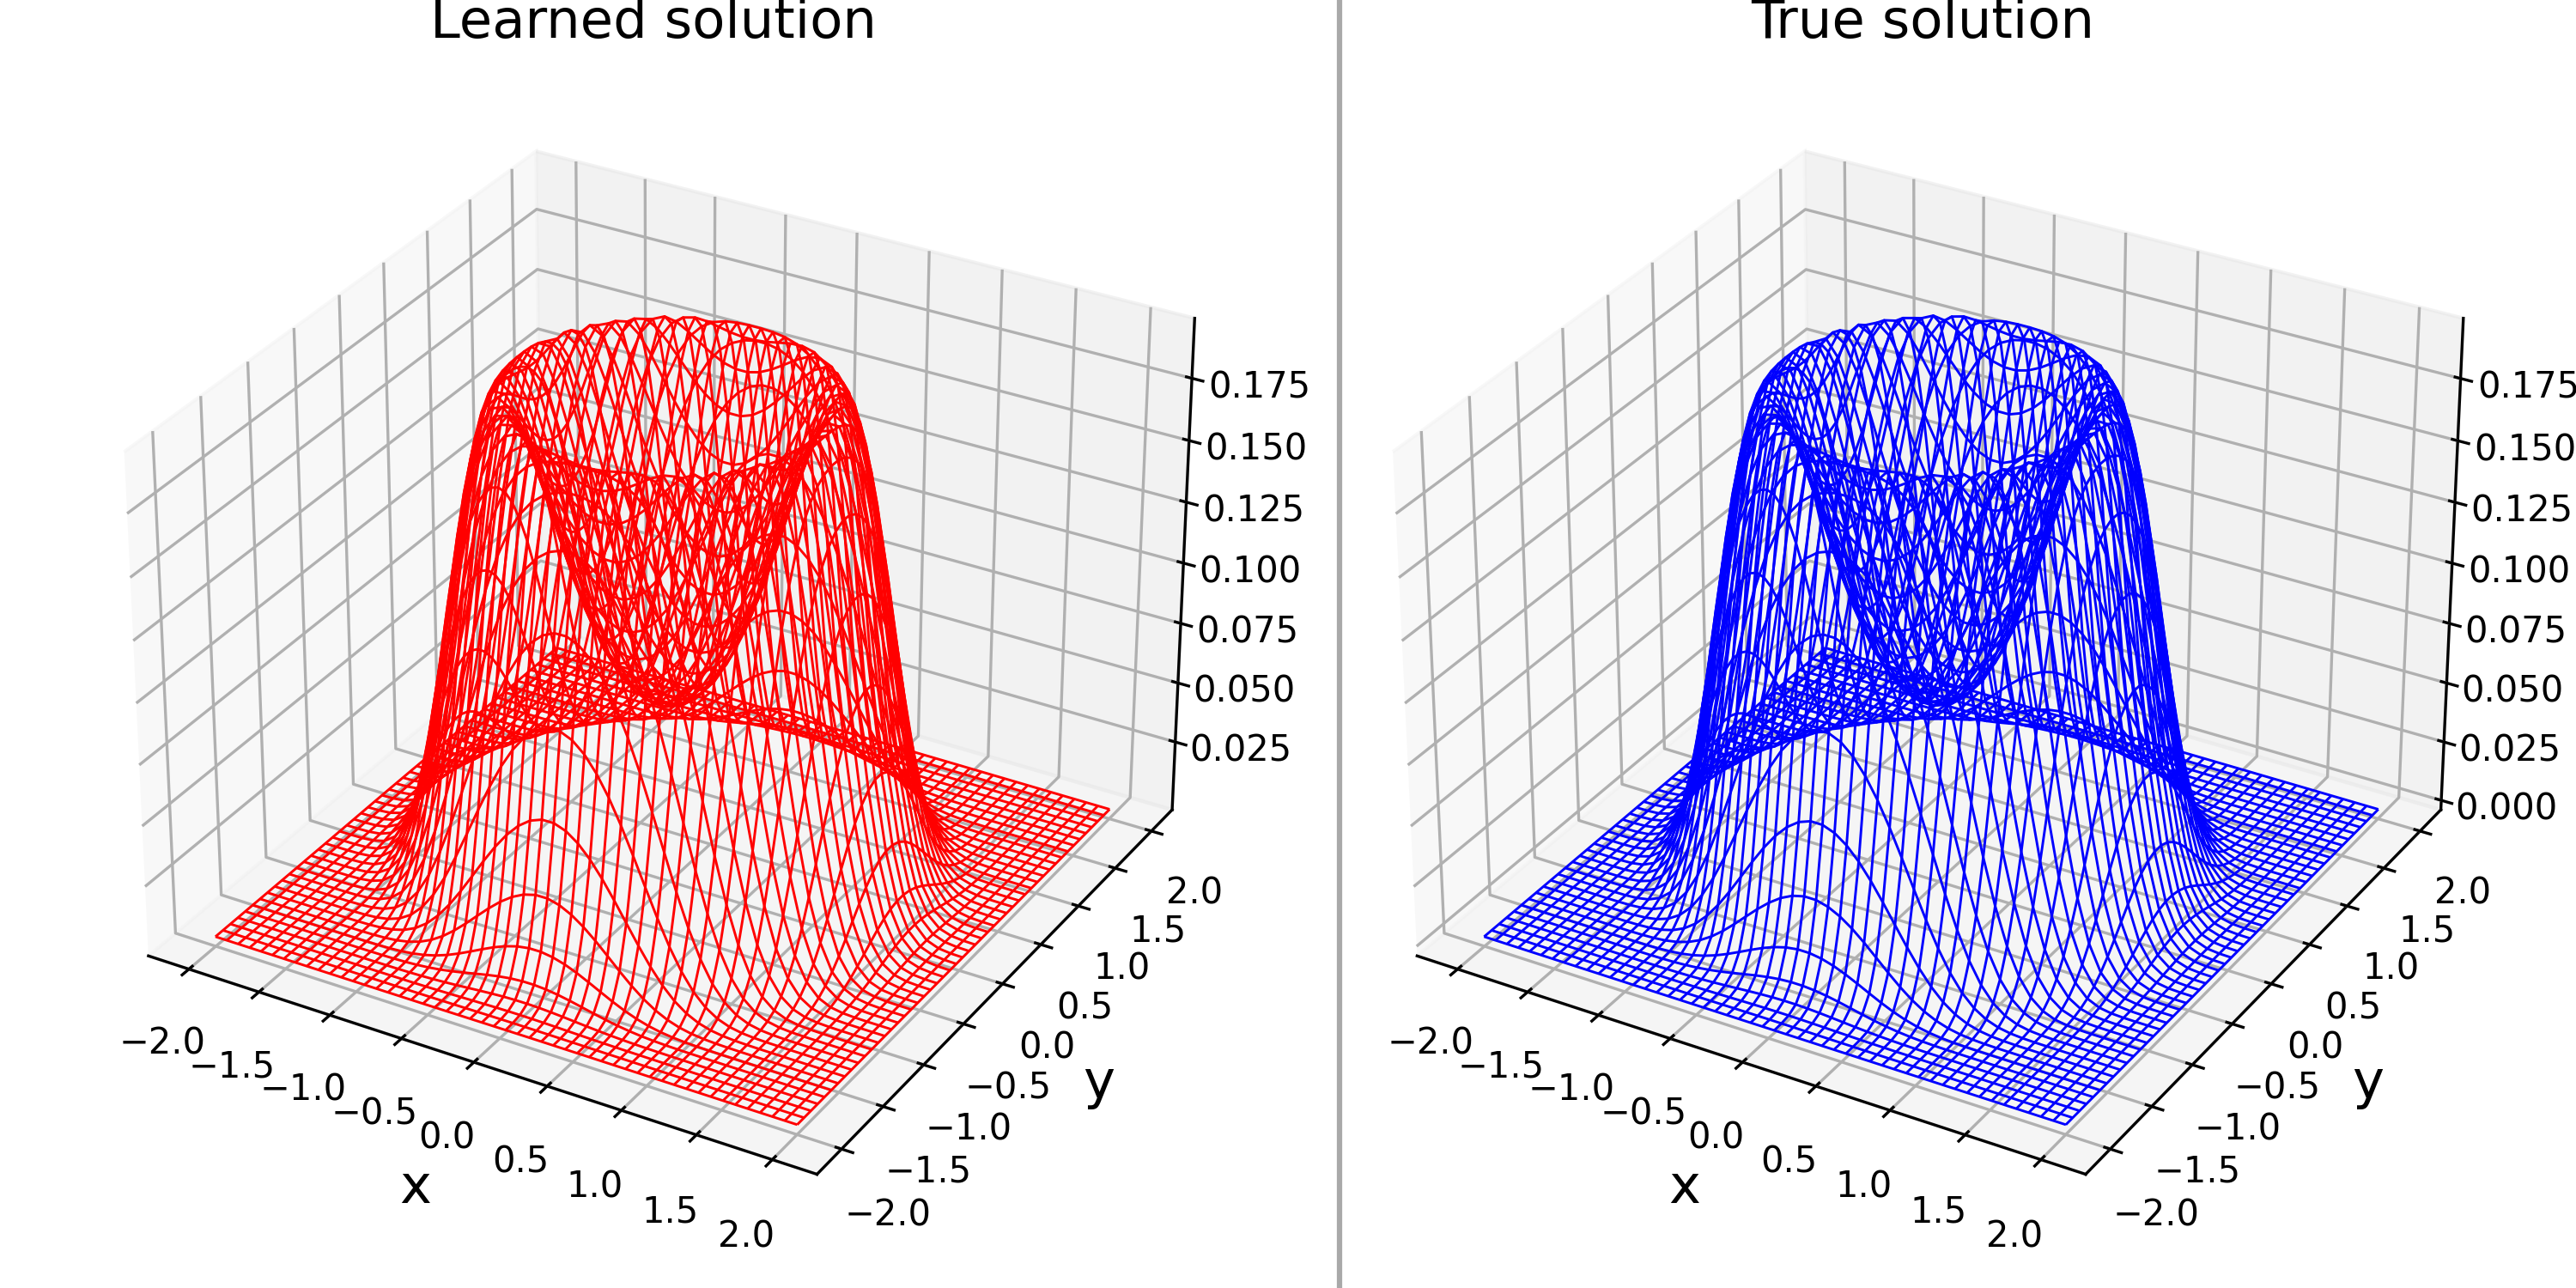
\includegraphics[scale=0.6
]{steady-fp/plots/2D-surface.png}
    \caption{Solution for the 2D ring system}
    \label{fig:2D-surface--steady-fp}
\end{figure}
In this case we use $\Omega_I=[-2,2]^2$ and $E=8\times10^5$ iterations. 
\subsubsection{Comparison with Monte Carlo}\label{sssec-MC-comparison--steady-fp} Since the network was trained with domain resampling every $10$ steps and a mini-batch size of $N=1000$, during the entire training procedure $8\times10^7$ points were sampled from the domain. We compute the steady state with Monte Carlo with $8\times10^7$ particles to compare errors produced by both methods. Here the SDE trajectories were generated till time 10 with time-steps of 0.01. Since in this case we know the analytic solution we can compute and compare absolute errors. As we can see in figure~\ref{fig:MC-comparison--steady-fp}, for the same number of overall sampled points, Monte Carlo error is an order of magnitude larger than deep learning error. 

\begin{figure}[!ht]
    \centering
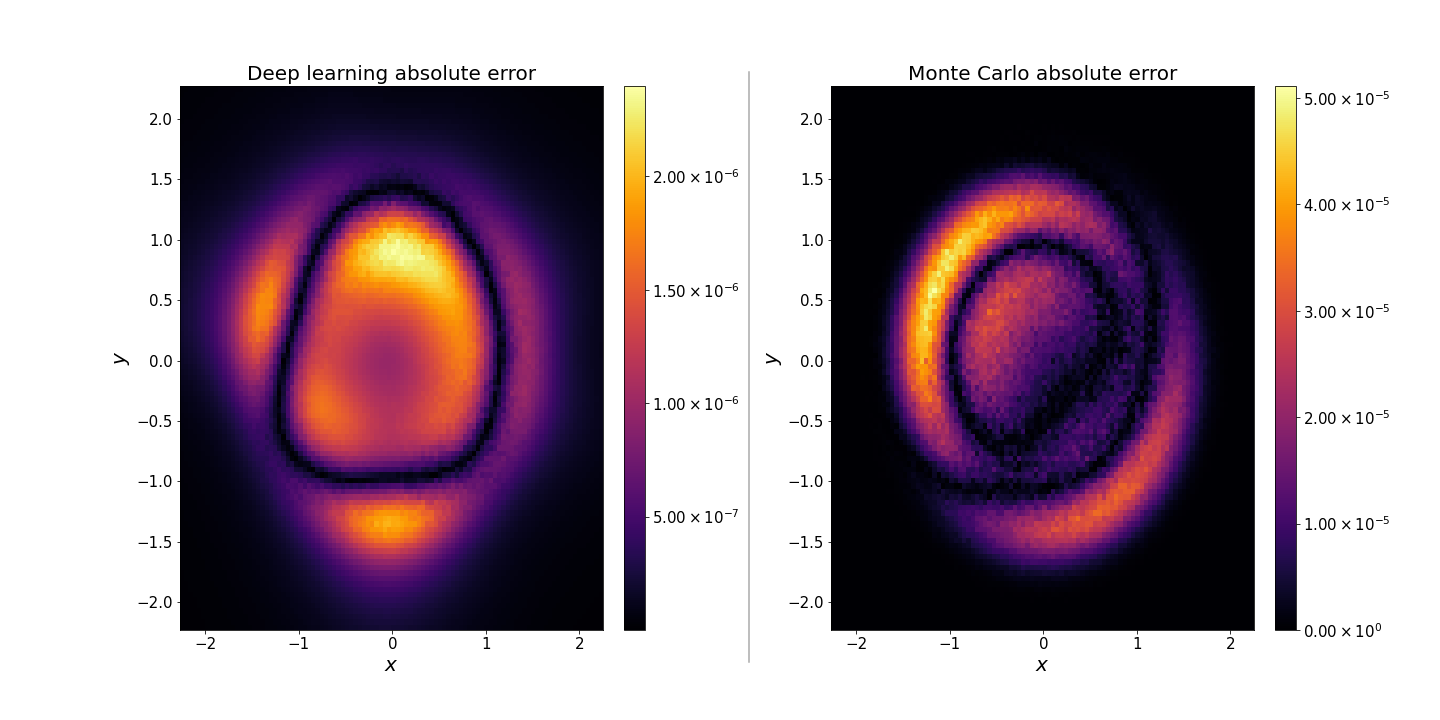
\includegraphics[scale=0.32]{steady-fp/plots/2D-error.png}
\caption{Comparison of absolute errors for deep learning and Monte Carlo solutions for the 2D ring system}
    \label{fig:MC-comparison--steady-fp}
\end{figure}

\subsection{2nD ring system}
Although we solve this system for $n=1,2,3,4,5$, in this section we only produce the results for $n=5$ or $d=10$ to avoid repetition. Figure~\ref{fig:10D-surface--steady-fp} shows the solutions for  the 10D ring system for $\Omega_I=[-2, 2]^{10}$ and $E=4.6\times10^6$. In order to visualize the solution we focus on the quantity
$
    p(0, 0, 0, 0, x_4, x_5, 0, 0, 0, 0)
$.
For a visual comparison with the true solution normalization is desirable. But rather than trying to compute a 10-dimensional integral which is a non-trivial problem in itself we can normalize $
    p(0, 0, 0, 0, x_4, x_5, 0, 0, 0, 0)
$ which is much easier to do and due to the decoupled nature of this problem we can expect an identical result as in figure~\ref{fig:2D-surface--steady-fp} which is what we see in figure~\ref{fig:10D-surface--steady-fp}. In both of the panels the solutions have been normalized in a way such that,
$$\int_{\mathbb R}\int_{\mathbb R}p(0, 0, 0, 0, x_4, x_5, 0, 0, 0, 0)\,dx_4\,dx_5=1$$

\begin{figure}[!ht]
    \centering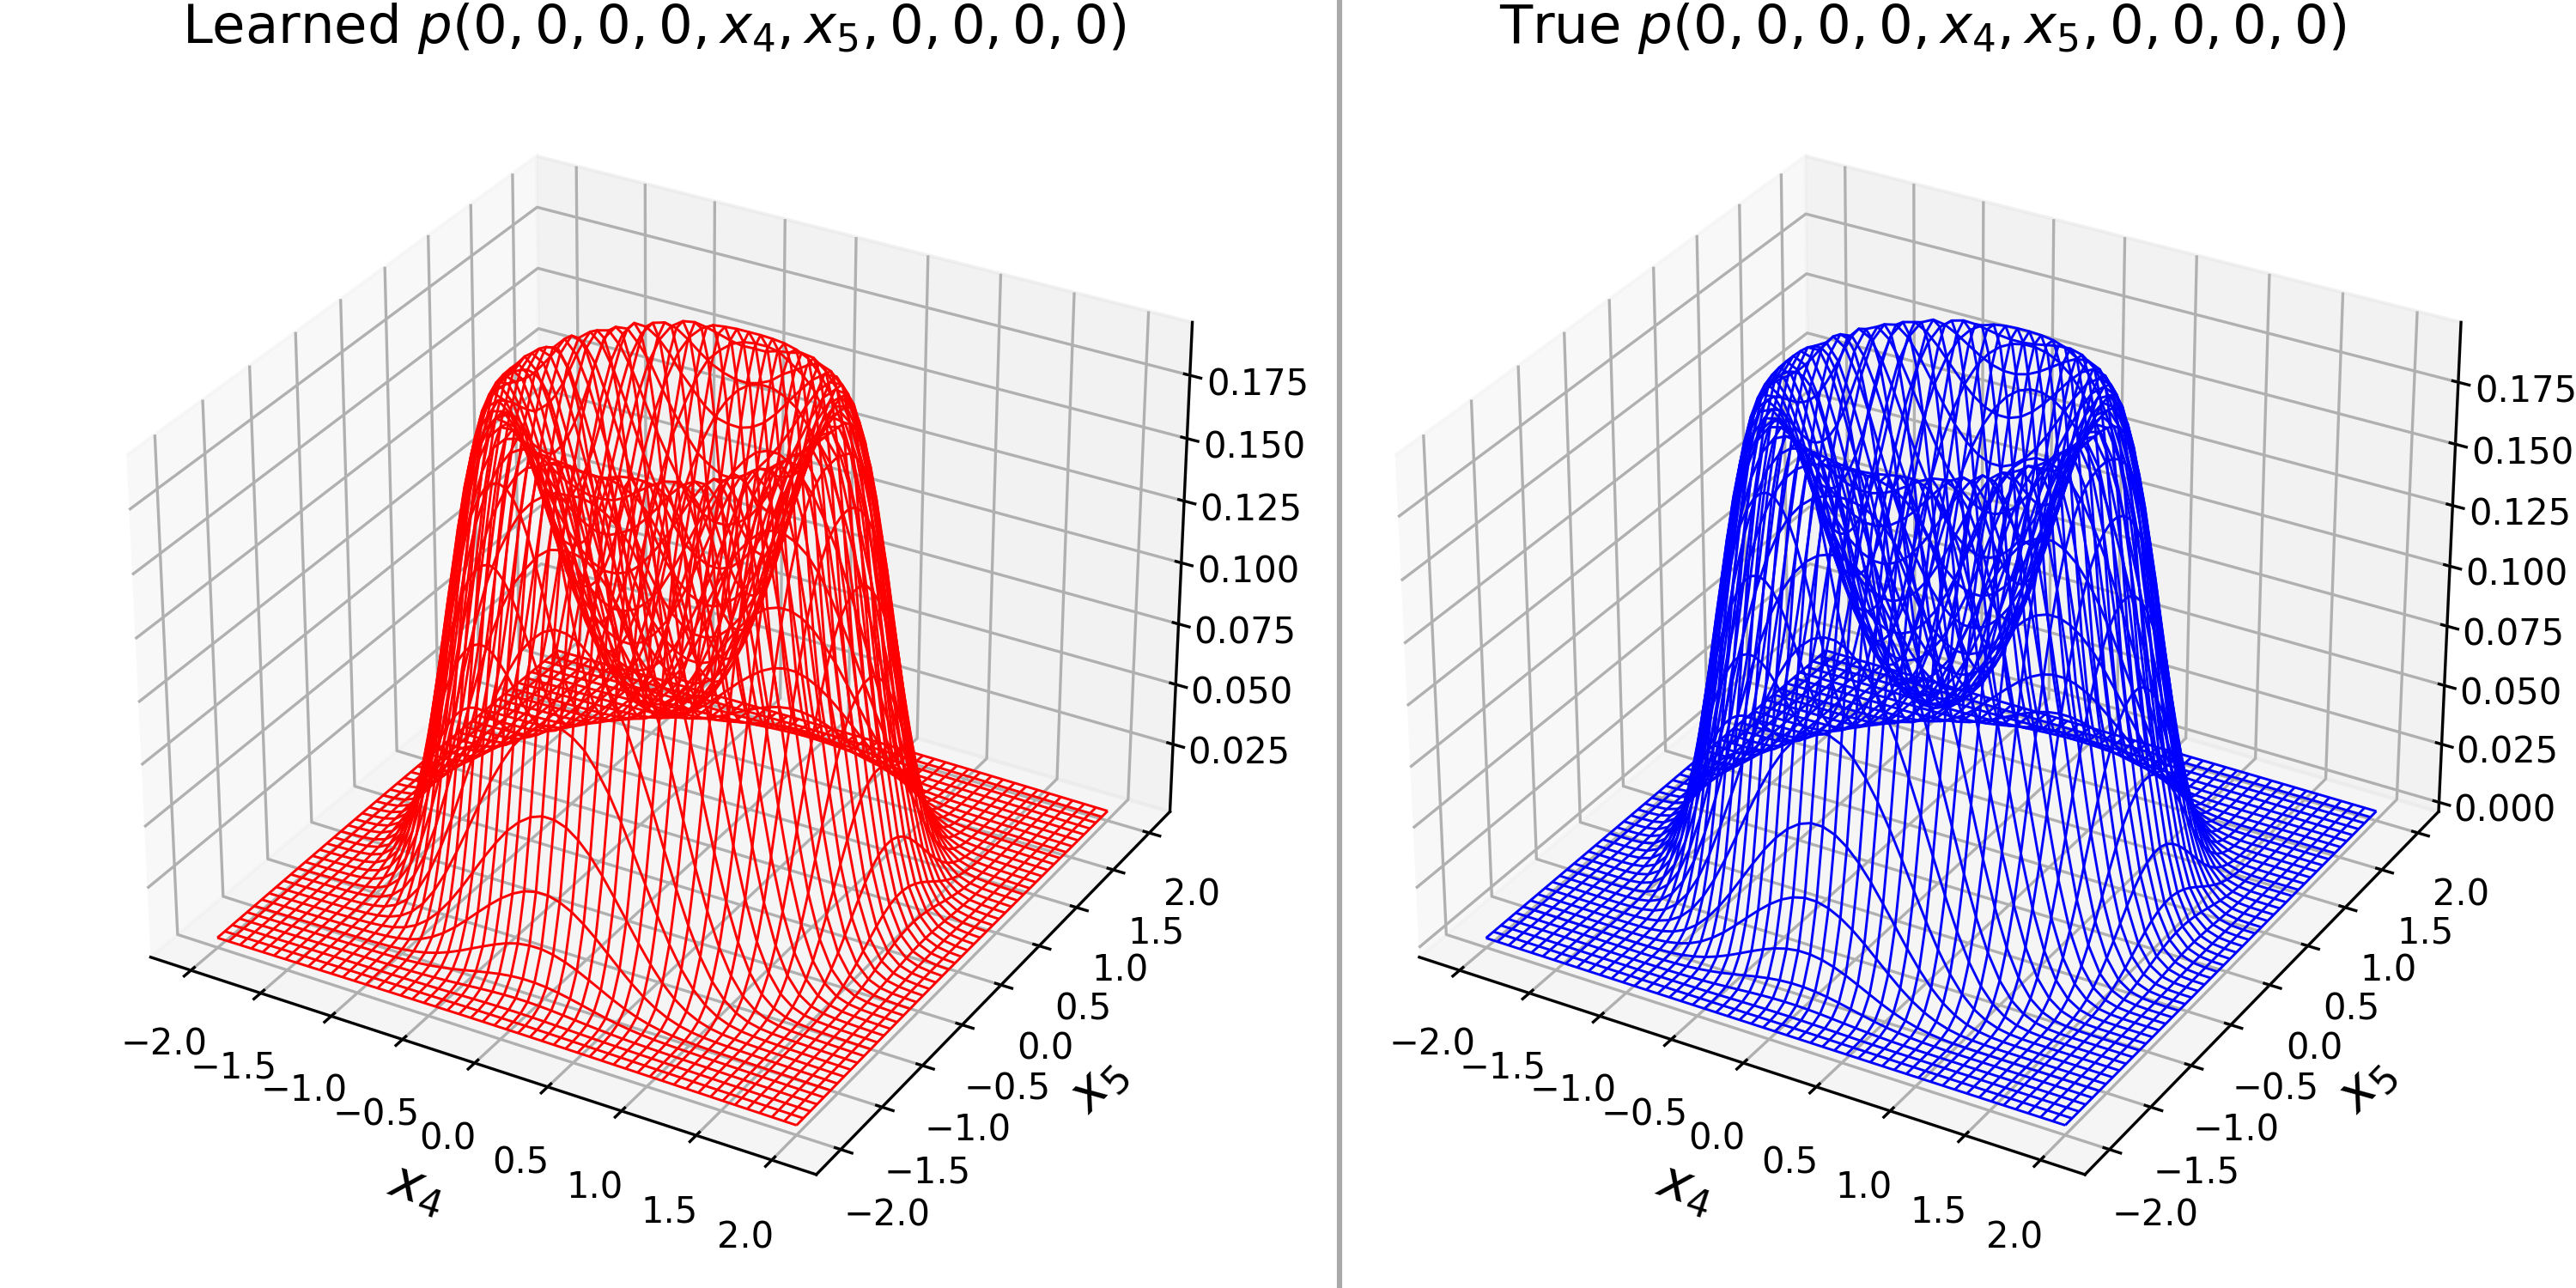
\includegraphics[scale=0.6
]{steady-fp/plots/10D-surface.png}
\caption{Solutions for the 10D ring system. Both solutions have been normalized such that $\int_{\mathbb R}\int_{\mathbb R}p(0, 0, 0, 0, x_4, x_5, 0, 0, 0, 0)\,dx_4\,dx_5=1$} 
    \label{fig:10D-surface--steady-fp}
\end{figure}
The error in the learned solution can be seen in figure~\ref{fig:10D-error--steady-fp}.

\begin{figure}[!ht]
    \centering
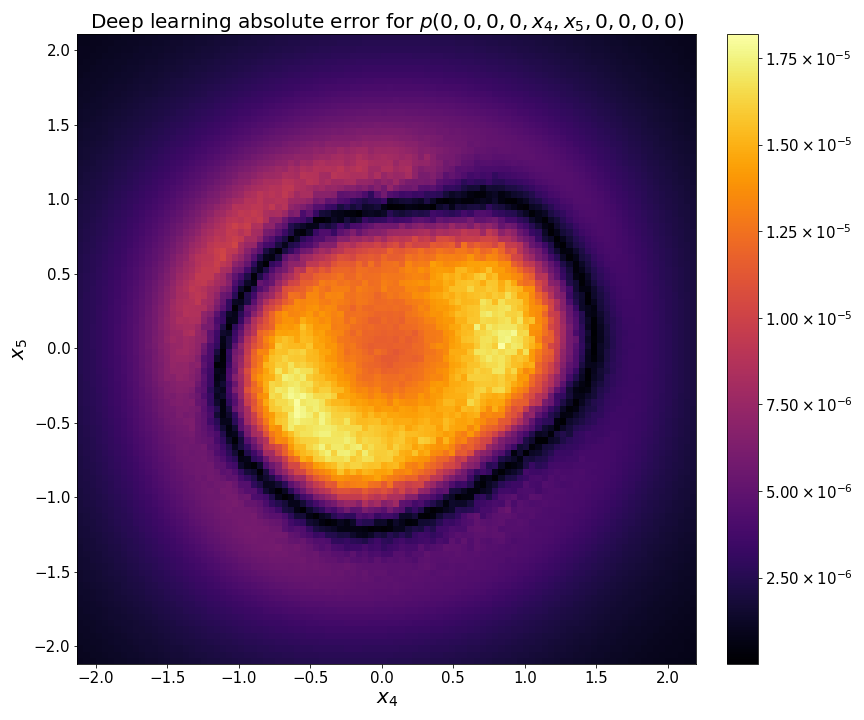
\includegraphics[scale=0.32]{steady-fp/plots/10D-error.png}
\caption{Absolute error in the learned solution for the 10D ring system}
    \label{fig:10D-error--steady-fp}
\end{figure}

    

\subsection{Noisy Lorenz-63 system} Figure~\ref{fig:L63-steady--steady-fp} shows the results for the L63 system for $\Omega_I = [-30, 30]\times[-40, 40]\times[0, 70]$ and $E=10^6$. For ease of visualization the solutions have been normalized and in each row one of the dimensions has been integrated over the relevant interval to produce 2D marginals. In order to integrate out one dimension we use a composite Gauss-Legendre quadrature rule. We subdivide the relevant interval into 240 subintervals and use 10-point Gauss-Legendre rule to compute the integral over every subinterval. Note that since $n_\theta$ is a smooth function, our integrand is always a smooth function. The largest possible subinterval is of length $\frac{40-(-40)}{240}=\frac{1}{3}$ so assuming absolute value of the $20$-th derivative of the integrand is upper-bounded by $M$ everywhere, the integration error on each subinterval is upper-bounded by $\frac{2M}{20!}\left(\frac{1}{6}\right)^{20}\le2.25M\times10^{-34}$, see appendix~\ref{ssec-error-GL--steady-fp} for more details on this estimate. To produce the Monte Carlo solution, SDE trajectories were generated till time 10 with time-steps of $10^{-2}$. 
Since Monte Carlo produces lower-accuracy solutions even in lower dimensions as we saw in section~\ref{sssec-MC-comparison--steady-fp} and an analytic solution is unavailable in this case, we refrain from producing error plots.

\begin{figure}[!ht]
    \centering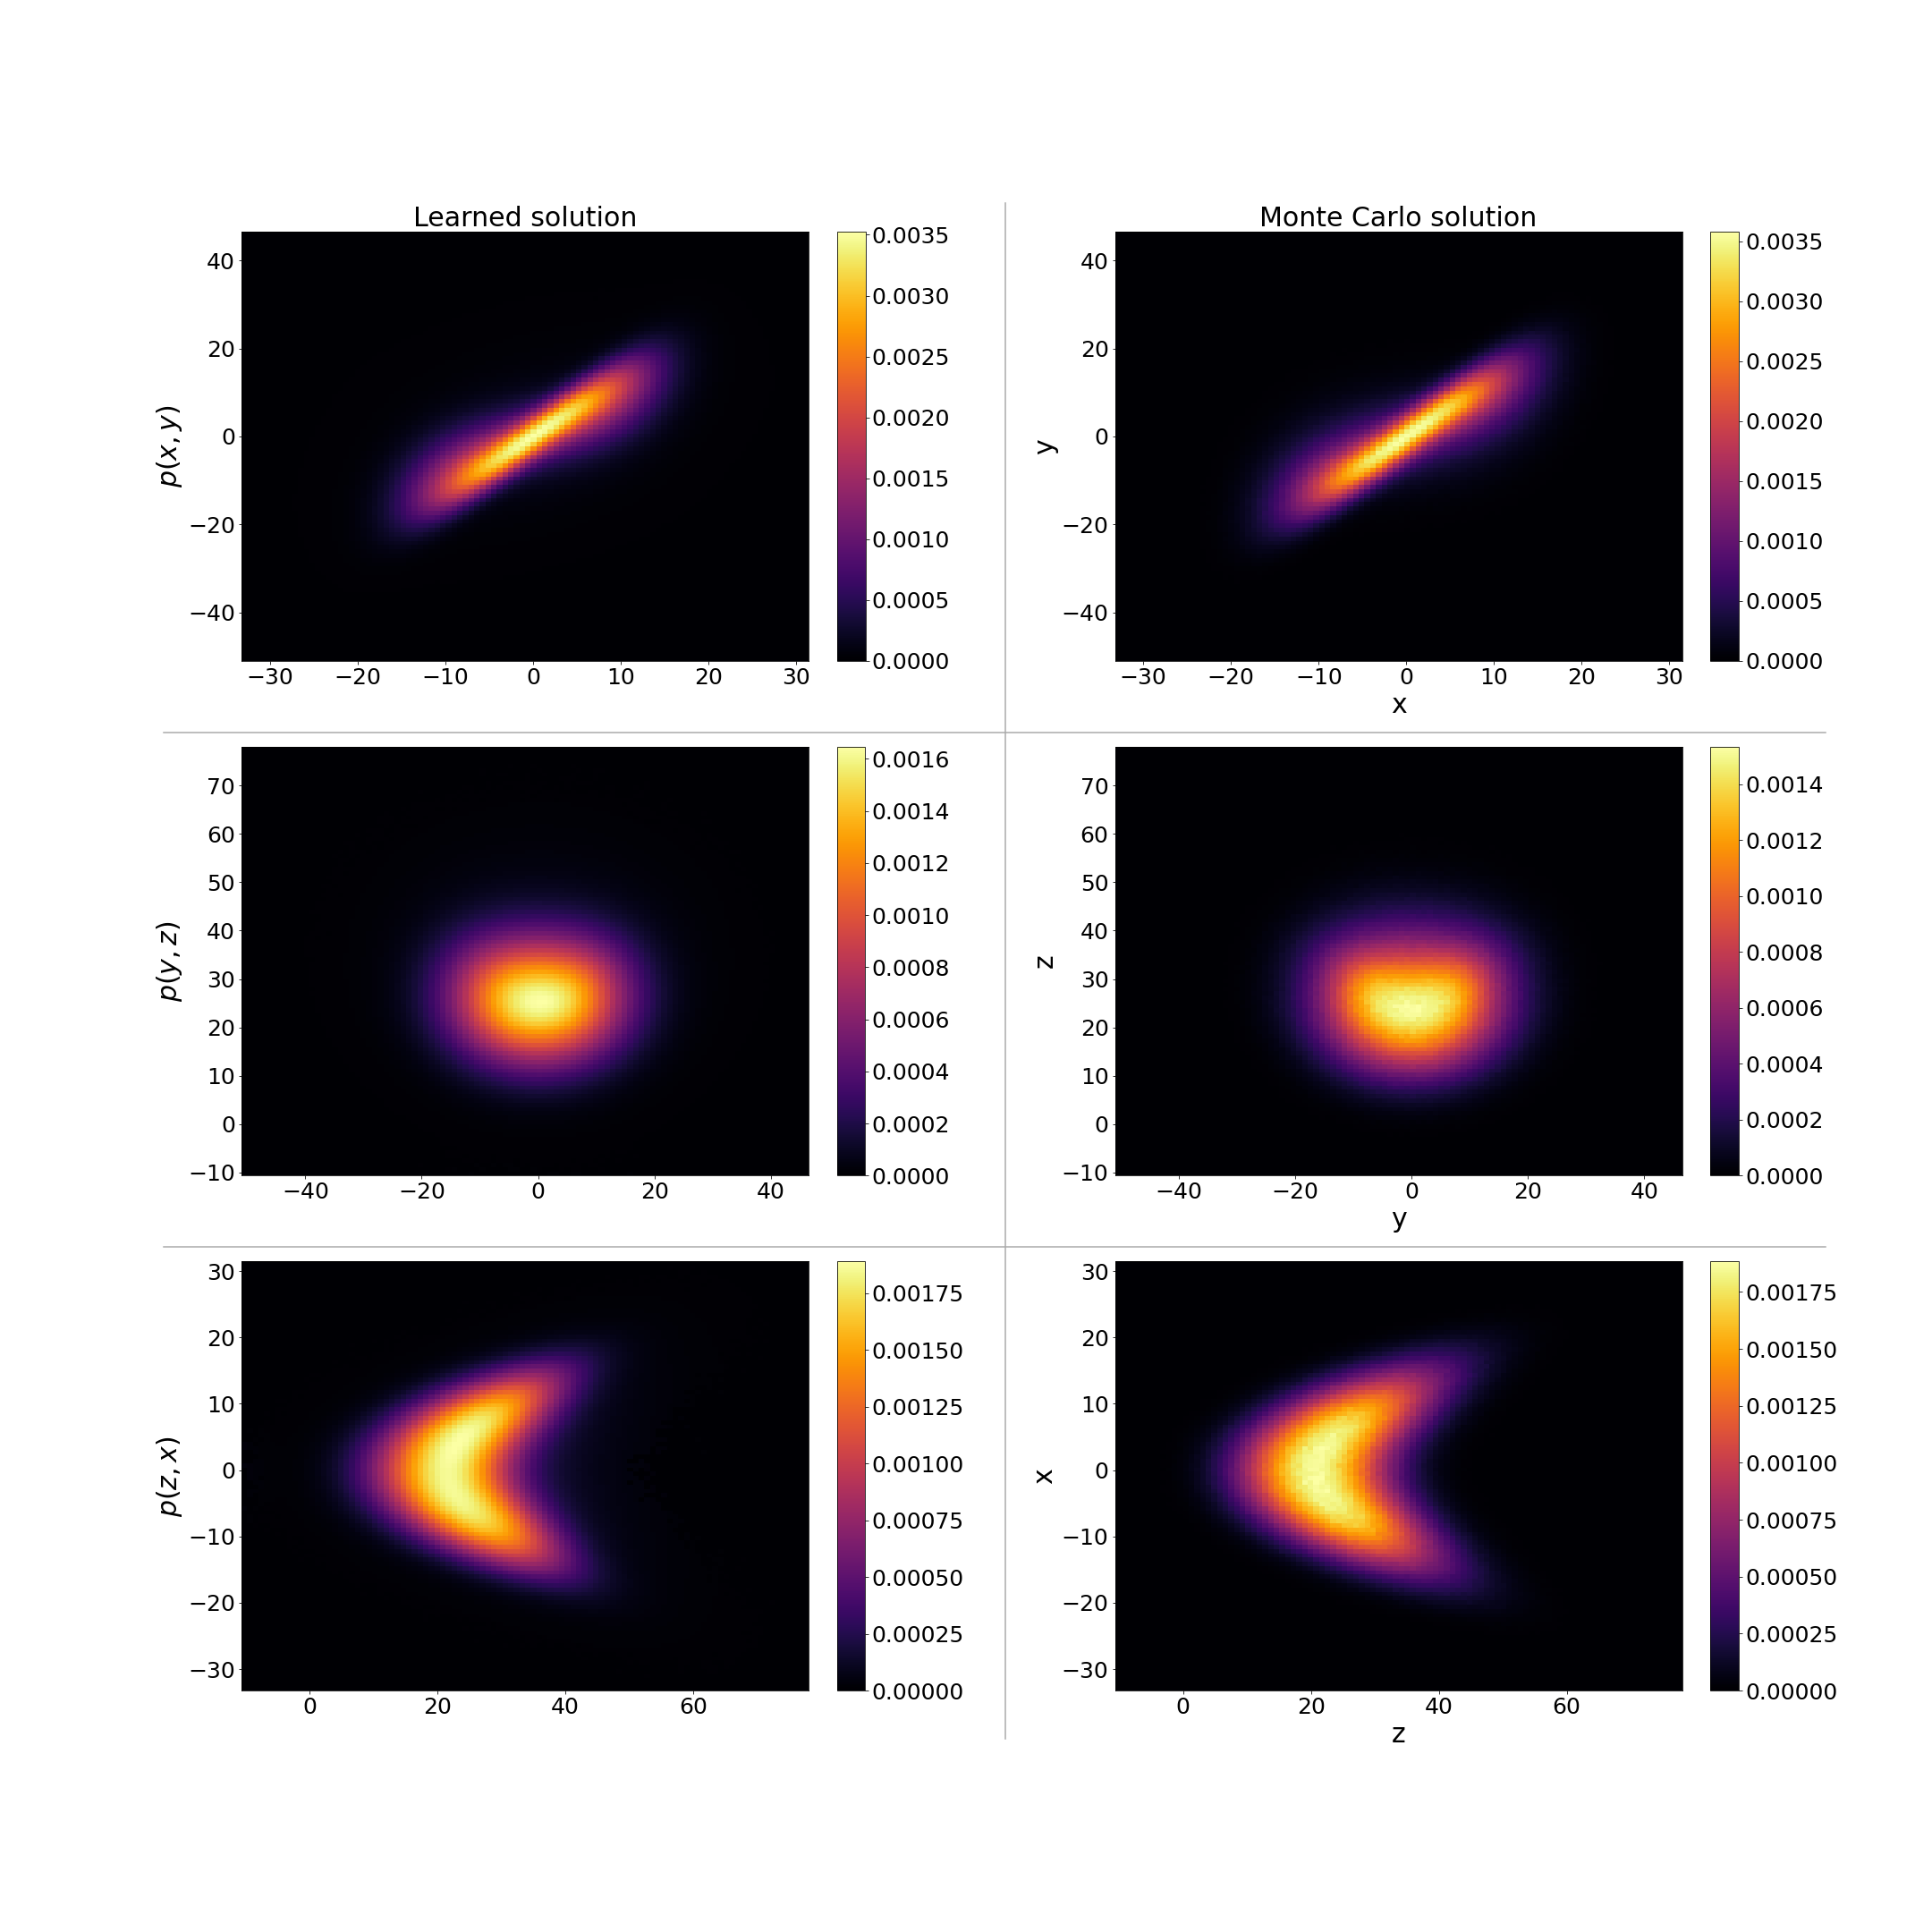
\includegraphics[scale=0.21]{steady-fp/plots/L63-steady.png}  \caption{Solutions for the noisy Lorenz-63 system}
    \label{fig:L63-steady--steady-fp}
\end{figure}

\subsection{Noisy Thomas system}
Figure~\ref{fig:Thomas-steady--steady-fp} shows the results for the Thomas system for $\Omega_I = [-10, 10]^3$ and $E=4\times10^5$. Due to the inherent symmetry of this problem it suffices to compute only the 2D marginal $p(x, y)$. To integrate out the $z$ dimension we use 8-point composite Gauss-Legendre quadrature rule with $165$ subintervals. Assuming absolute value of the $16$-th derivative of the integrand is upper-bounded by $M$ everywhere, the integration error on each subinterval is upper-bounded by $\frac{2M}{16!}\left(\frac{10}{165}\right)^{16}\le3.17M\times10^{-33}$, see appendix~\ref{ssec-error-GL--steady-fp} for more details on this error estimate. To produce the Monte Carlo solution, SDE trajectories were generated till time 10 with time-steps of $10^{-2}$. Even though we have solved a lower dimensional problem here, Thomas system turns out to be the \textit{easiest} i.e. algorithm~\ref{algo:steady--steady-fp} converges faster for this system compared to the other ones as we will see in the next section.
\begin{figure}[!htp]
    \centering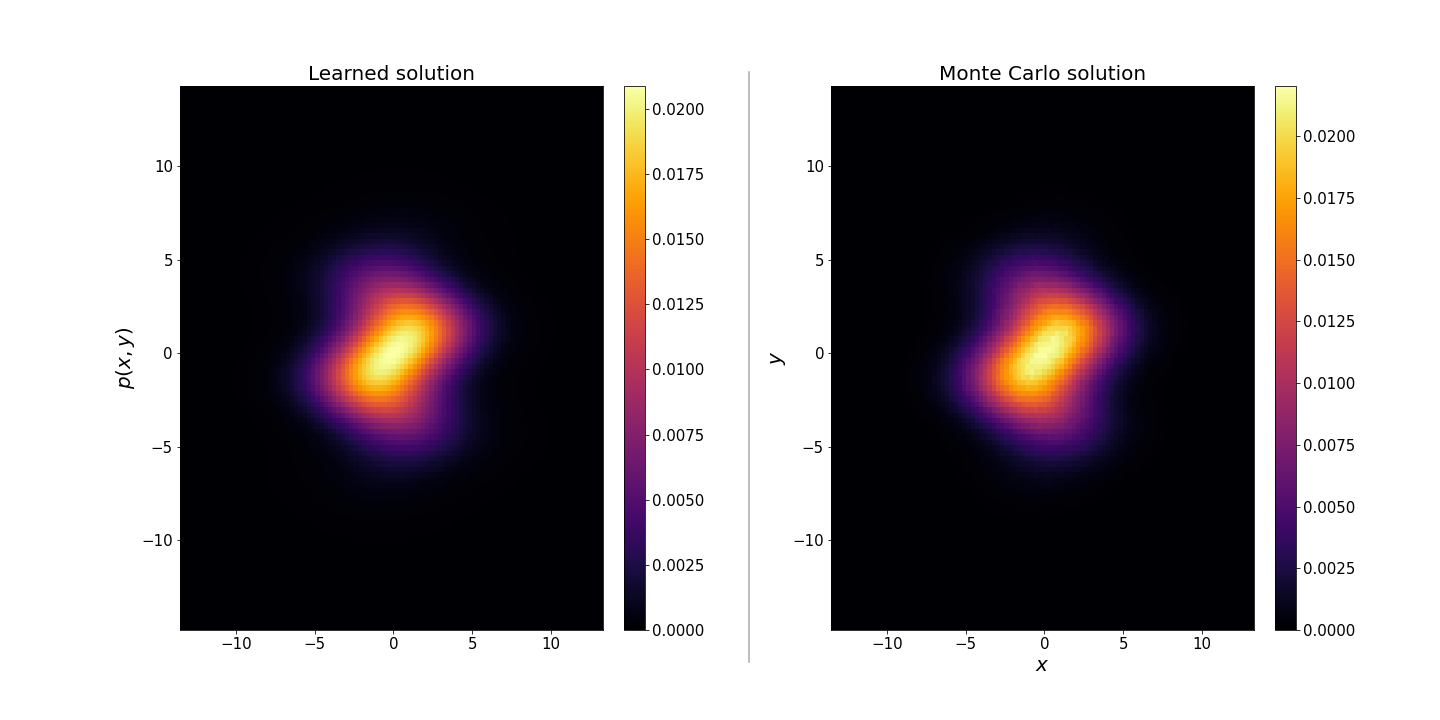
\includegraphics[scale=0.32]{steady-fp/plots/Thomas-steady.png}
    \caption{Solutions for the noisy Thomas system}
    \label{fig:Thomas-steady--steady-fp}
\end{figure}
\subsection{Dimension dependence} In this section we explore the dimension dependence of algorithm~\ref{algo:steady--steady-fp}.
In the left panel of figure~\ref{fig:time-loss--steady-fp} we have plotted the loss given by \eqref{eq:def-steady-loss--steady-fp} against training iterations for all the of the systems above in a semi-log manner starting from iteration $100$. We often encounter spikes in the loss curve for the following reasons
\begin{itemize}
    \item the loss curves are single realizations of algorithm~\ref{algo:steady--steady-fp} instead of being an average
    \item we resample the domain every $10$ iterations and if the new points belong to a previously unexplored region in $\Omega_I$, the loss might increase.
\end{itemize}
But the general trend of loss diminishing with iterations is true for every system. We also see that loss is system-dependent and the \textit{hardness} of these problems or how quickly algorithm~\ref{algo:steady--steady-fp} converges depends on the nature of $\mu$ as much as the dimension. This is easily seen by noting that the two 3D systems sandwich the 2D and the 4D ring systems in the left panel of figure~\ref{fig:time-loss--steady-fp}. The loss for Thomas system drops very quickly compared to the rest of the systems due to the simplicity and global Lipschitzness of the corresponding drift function. We also see from the right panel of figure~\ref{fig:time-loss--steady-fp} that time taken per training iteration grows near-linearly with dimension. Since it is hard to estimate the amount of iterations to run before the loss drops below a pre-determined level, we refrain from plotting the total runtime of algorithm~\ref{algo:steady--steady-fp} against dimension. But it's interesting to note that the number of total training iterations $E$ varies from $4\times10^5$ to $4.6\times10^6$ across all the problems. Since the data shown in the right panel of figure~\ref{fig:time-loss--steady-fp} is very much hardware dependent, at this point we disclose that all of the experiments were done using the cloud service provided by Google Colab. This service automatically assigns runtimes to different hardware depending on availability at the time of computation which might explain why the 8D and 10D ring systems take nearly the same amount of time per iteration in figure~\ref{fig:time-loss--steady-fp}.
\begin{figure}[!ht]
    \centering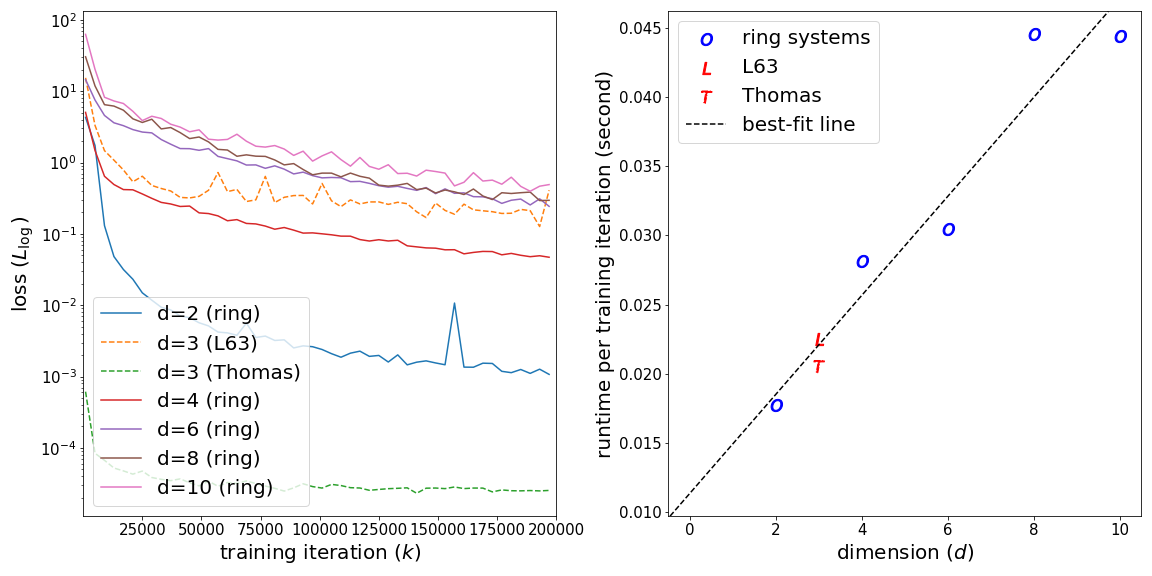
\includegraphics[scale=0.4]{steady-fp/plots/loss-time.png}
    \caption{Left panel: Loss vs training iteration starting from iteration $100$. Right panel: time taken per training iteration vs dimension.}
    \label{fig:time-loss--steady-fp}
\end{figure}
\subsection{Comparison of loss and distance from truth} In this section we explore the relationship between the loss given by \eqref{eq:def-steady-loss--steady-fp} and the distance from truth. In spite of being structurally completely different, both are measures of goodness for a computed solution. In most cases we only have access to the loss and therefore it is an important question if a decreasing loss implies getting closer to the truth for algorithm~\ref{algo:steady--steady-fp}. We define the distance of the learned zero from the true solution as follows,
\begin{align}
    \|\phi\|_*\stackrel{\rm def}{=}\sup_{\mathbf x\in\Omega_I} |c\phi(\mathbf x) - p^{\rm true}(\mathbf x)|\label{eq:def-sup-norm--steady-fp}, \qquad c\int_{\mathbb R^d}\phi=1
\end{align}
where $p^{\rm true}$ is the true solution to \eqref{eq:SFPE-0--steady-fp}. \eqref{eq:def-sup-norm--steady-fp} is not easy to compute in arbitrary dimensions but can be computed for the 2D ring system without too much effort since $p^{\rm true}$ is known and the problem is low-dimensional. Figure~\ref{fig:dist-loss--steady-fp} shows the results for the 2D ring system. The right panel of figure~\ref{fig:dist-loss--steady-fp} shows that loss and distance from truth are strongly correlated for algorithm~\ref{algo:steady--steady-fp}. Moreover, asymptotically for small values of the loss function they are linearly related with a Pearson correlation coefficient $R=0.98$ as can be seen from the inset in the right panel which depicts the data from training iteration 10000 to 50000. The best-fit line is also shown in the inset. On the left panel we see that the distance from truth monotonically decreases with training iteration and is extremely well approximated by a curve of the form $a_0e^{-a_1k}+a_2$. Both panels contain data from training iteration 5000 to 50000. We omit the first few iterations to filter out the effects of the random initialization of the trainable parameters. Figure~\ref{fig:dist-loss--steady-fp} serves as a good justification for algorithm~\ref{algo:steady--steady-fp} since it shows that minimizing the loss is akin to getting closer to a true non-trivial zero of $\mathcal L$.
 
\begin{figure}[!ht]
    \centering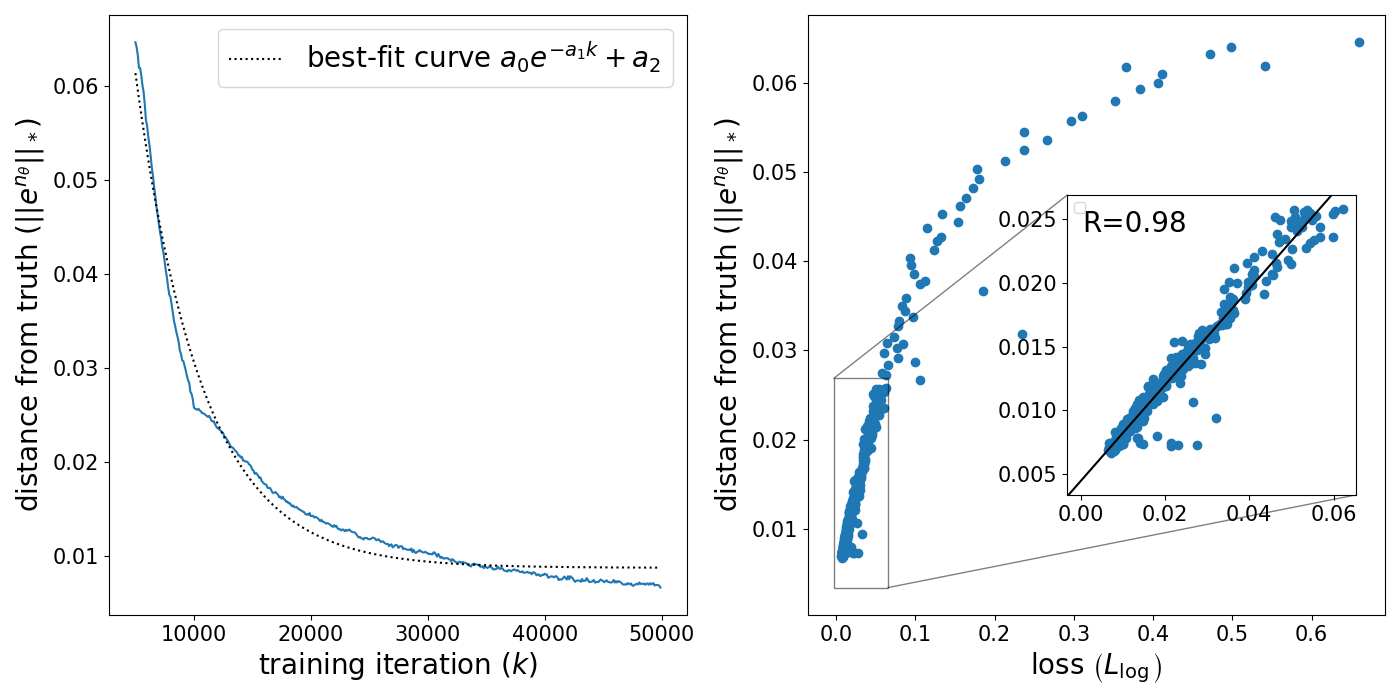
\includegraphics[scale=0.4]{steady-fp/plots/2D-distance.png}
    \caption{Left panel: Distance from truth vs training iteration every 100 iterations, starting from iteration 5000 and ending at iteration 50000 for the 2D ring system. Right panel: Scatter plot for loss vs distance from truth for the 2D ring system. The inset shows that asymptotically loss and the distance from the truth are linearly related. The inset depicts the data from training iteration $10000$ to $50000$.}
    \label{fig:dist-loss--steady-fp}
\end{figure}


\section{Conclusions and future work}
\label{sec-conclusions--steady-fp}
In this work we devise a deep learning algorithm  for finding non-trivial zeros of $\mathcal L$ when the corresponding drift is non-solenoidal. We can summarize our results as follows. 
\begin{enumerate}
    \item Our choice of architecture is capable of learning zeros of Fokker-Planck operators across many different problems while scaling only linearly with dimension.
    \item Time taken per training iteration grows near-linearly with problem dimension.
    \item Apart from being able to produce solutions in a functional form which Monte Carlo is incapable of, for the same overall sample-size algorithm~\ref{algo:steady--steady-fp} produces more accurate solutions compared to Monte Carlo.
    \item How quickly algorithm~\ref{algo:steady--steady-fp} converges to a zero depends as much on the dimension as it does on the nature of the problem or the structure of $\mu$.
    \item By minimizing the loss we also get closer to a true non-trivial zero of the Fokker-Planck operator which justifies algorithm~\ref{algo:steady--steady-fp}.
    \item The loss and the distance from a true zero of the Fokker-Planck operator, even though structurally completely different, are strongly correlated. Moreover, they can be asymptotically linearly related for small values of the loss function.
\end{enumerate}
In a sequel we will show how we can solve time-dependent FPEs by using the zeros learned by algorithm~\ref{algo:steady--steady-fp}. The landscape of the loss defined in \eqref{algo:steady--steady-fp} poses many interesting geometric questions. For example, in case the nullspace of $\mathcal L$ is 1-dimensional do all the minima of $L_{\log}$ lie on a connected manifold of dimension $1$
or are they disconnected from each other? Such questions provide possible avenues for future research.


\section{Appendix}
\label{sec-appendix--steady-fp}
\subsection{Existence and uniqueness of solutions to example problems}\label{ssec-unique--steady-fp} In this section we prove that the example problems used here have a unique weak solution in $W^{1,2}_{\rm loc}(\mathbb R^d)$.
 We employ the method of Lyapunov function as described in \cite{huang2015steady} to arrive at existence and uniqueness. First we begin with the prerequisites for this approach.
 \subsubsection{Lyapunov functions}
\begin{defn}
    Let $U \in C(\mathcal U)$ be a non-negative function and denote $\rho_M = \sup_{\mathbf x\in \mathcal U} U(\mathbf x)$,
called the essential upper bound of $U$. $U$ is said to be a compact function in $U$ if
\begin{align}
i)\; U (\mathbf x) < \rho_M,\quad \mathbf x \in \mathcal U
\end{align}
and
\begin{align}
ii) \lim_{\mathbf x\to\partial U} U (\mathbf x) = \rho_M 
\end{align}
\end{defn} This definition of a compact function appears as definition 2.2 in \cite{huang2015steady}.
\begin{prop}
An unbounded, non-negative function $U\in C(\mathbb R^d)$ is compact iff 
\begin{align}
    \lim_{\|\mathbf \mathbf x\|_2\to+\infty} U(\mathbf x) = +\infty
\end{align}
\end{prop}
This proposition appears as proposition 2.1 in \cite{huang2015steady}.

\begin{defn}
    Let $U$ be a compact function in $C^2(\mathcal U)$ with essential upper bound $\rho_M$. $U$ is called a Lyapunov function in $\mathcal U$ with respect to $\mathcal L^*$ is $\exists\,\rho_m\in(0, \rho_M)$ and a constant $\gamma>0$ such that
    \begin{align}
        \mathcal L^* U(\mathbf x)\le -\gamma,\qquad\forall \mathbf x\in \mathcal U\setminus\overline{\{\mathbf x\in\mathcal U: U(\mathbf x)<\rho_m\}}
    \end{align}
    where $\mathcal L^*$ is the adjoint Fokker-Planck operator given by
    \begin{align}
        \mathcal L^*f = \mu\cdot\nabla f+ D\odot\nabla^2 f \label{eq:def-adjoint-FP-op--steady-fp}
    \end{align}
\end{defn}
This definition appears as definition 2.4 in \cite{huang2015steady}.
Now we are ready to state the main theorem that will help us prove uniqueness for our example problems.
\begin{thm}
    If the components of $\mu$ are in $L^2_{\rm loc}(\mathcal U)$ and there exists a Lyapunov function with respect to $\mathcal L^*$ in $C^2(\mathcal U)$ then \eqref{eq:SFPE-0--steady-fp} has a positive weak solution in the space $W^{1, 2}_{\rm loc}(\mathcal U)$. If, in addition,
the Lyapunov function is unbounded, the solution is unique in $\mathcal U$.\label{thm:unique-steady--steady-fp}
\end{thm}
This theorem appears as theorem $A$ in \cite{huang2015steady}. Since the components of $\mu$ are locally integrable for our example problems, all we need to do is find an unbounded Lyapunov function $U$ for proving existence and uniqueness in $W^{1,2}_{\rm loc}(\mathbb R^d)$.
\subsubsection{Existence and uniqueness of solution for 2D ring system}\label{sssec-2D-unique--steady-fp}
Setting 
\begin{align}
\mathcal U &= \mathbb R^2\\
U(x, y) &= x^2+y^2\\
\rho_m &= \frac{1}{2}+\sqrt{D+1}\\
\gamma &= 4D+6\\
\end{align}
we see that,
\begin{align}
    \mathcal L^*U +\gamma = -8\left(x^2+y^2-\frac{1}{2}\right)^2 + 8(D+1)
\end{align}
and,
\begin{align}
    \mathcal U\setminus\overline{\{\mathbf x\in\mathcal U: U(\mathbf x)<\rho_m\}} = \left\{(x,y)\in\mathbb R: x^2+y^2>\rho_m\right\}
\end{align}
In  $\left\{(x,y)\in\mathbb R: x^2+y^2>\rho_m\right\}$, 
\begin{align}
    \mathcal L^*U+\gamma \le 0
\end{align}
and therefore $U$ is an unbounded Lyapunov function for the 2D ring system which guarantees uniqueness of solution \eqref{eq:grad-sol--steady-fp}.

\subsubsection{Existence and uniqueness of solution for L63 system}\label{sssec-L63-unique--steady-fp}
Setting,
\begin{align}
U(x, y, z) = \rho x^2 +\alpha y^2 + \alpha(z-2\rho)^2
\end{align}
we see that
\begin{align}
    \mathcal L^*U &= -2\alpha\rho x^2 - 2\alpha y^2 -2\alpha\beta z^2 + 4\alpha\beta\rho z + 2D(2\alpha+\rho)\\
    &=-2\alpha\rho x^2 - 2\alpha y^2 -\alpha\beta z^2 -\alpha\beta(z-2\rho)^2 + 4\alpha\beta\rho^2 + 2D(2\alpha+\rho)\\
    &\le -\rho x^2 -\alpha y^2 -\alpha(z-2\rho)^2 + 4\alpha\beta\rho^2 + 2D(2\alpha+\rho)\label{eq:L63-params-bigger-than-1--steady-fp}\\
    &= -U(x, y, z)+ 4\alpha\beta\rho^2 + 2D(2\alpha+\rho)
\end{align}
\eqref{eq:L63-params-bigger-than-1--steady-fp} is a consequence of $\alpha, \beta, \rho>1$. Now setting,
\begin{align}
    \gamma &= 1,\\
    \rho_m &= 4\alpha\beta\rho^2 + 2D(2\alpha+\rho)+1
\end{align} we see that in $\{U>\rho_m\}$,
\begin{align}
    \mathcal L^*U +\gamma \le 0
\end{align}
So $U$ is an unbounded Lyapunov function for this system and we have a unique solution.
\subsubsection{Existence and uniqueness of solution for Thomas system}\label{sssec-Thomas-unique--steady-fp}
Setting,
\begin{align}
    U(x, y, z) = x^2+y^2+z^2
\end{align}
we see that
\begin{align}
    \mathcal L^* U &= x\sin y + y\sin z + z\sin x - b(x^2+y^2+z^2) + 6D\\
    &\le \sqrt{3U}-bU + 6D\label{eq:CS-on-Thomas-unique--steady-fp}\\
    &= -b\left(\sqrt{U}-\frac{\sqrt{3}}{2b}\right)^2 +\frac{3}{4b}+6D
\end{align}
\eqref{eq:CS-on-Thomas-unique--steady-fp} follows from Cauchy Schwarz inequality. Setting,
\begin{align}
    \gamma &= \frac{1}{4b},\\
    \rho_m &= \left(\frac{\sqrt{3}}{2b}+\frac{\sqrt{1+6bD}}{b}\right)^2
\end{align}
we see that in $\{U>\rho_m\}$,
\begin{align}
    \mathcal L^*U +\gamma \le 0
\end{align}
So $U$ is an unbounded Lyapunov function for this system and we have a unique solution.

\subsection{Monte Carlo steady state algorithm}\label{ssec-MC-algo--steady-fp}
The time-dependent FPE given by 


\begin{equation}
\begin{aligned}
    &\frac{\partial  p(t, \mathbf x)}{\partial t} =\mathcal L p(t, \mathbf x),\qquad\mathbf x\in\mathbb R^d,\; t\ge0\\&p(0, \mathbf x)=p_0(\mathbf x),\qquad\mathbf x\in\mathbb R^d\\
    &\int_{\mathbb R^d}p(t,\mathbf x)\,d\mathbf x = 1,\qquad\forall\;t\ge0
    \label{eq:FPE-0--steady-fp}
\end{aligned}
\end{equation}


gives us the probability density of the random process $X_t$ which is governed by the SDE,
\begin{equation}
\begin{aligned}
    &dX_t=\mu\,dt+\sigma\,dW_t\\
    &X_0\sim p_0\label{eq:SDE-0--steady-fp}
\end{aligned}
\end{equation}where $\{W_t\}$ is the standard Wiener process, see for example chapters 4, 5 of \cite{gardiner2009stochastic}. We can evolve $\eqref{algo:steady--steady-fp}$ up to sufficiently long time using Euler-Maruyama method \cite{kloeden1992stochastic} to approximate the steady state solution of \eqref{eq:FPE-0--steady-fp} or the solution of \eqref{eq:SFPE-0--steady-fp} as follows. Here $\mathcal N$ denotes the multivariate normal distribution.
%%%%%%
\begin{algorithm}[!ht]
Sample $\{ X_0^{(i)}\}_{i=1}^N\sim p_0$.\\
Set the time-step $h$.\\
Set the number of steps $S$.\\
\For {$k=1,2\cdots, S$}{
 Sample $w^i_k\sim\mathcal N(\mathbf 0_d, h I_d)\;\;\forall\;i$\\
 $ X_k^{(i)}\leftarrow  X_{k-1}^{(i)} + \mu\left(X_{k-1}^{(i)}\right)h + \sigma w_k^i\;\;\forall\;i$\\
}
Subdivide the domain of interest $\Omega_I$ into $d$-dimensional boxes.\\ Count the number of $X^{(i)}_{S}$ that are in a box to estimate the stationary density at the center of the box.
\caption{Monte Carlo steady state algorithm}\label{algo:MC--steady-fp}
\end{algorithm}
%%%%%%
Note that in case of a unique solution of \eqref{eq:SFPE-0--steady-fp}, many choices of $p_0$ can lead to the stationary solution. In all our examples, it suffices to choose $p_0$ to be the standard $d$-dimensional normal distribution.

\subsection{Integration error for \texorpdfstring{$n$}{Lg}-point Gauss-Legendre rule}\label{ssec-error-GL--steady-fp}
Suppose we are trying to integrate a smooth function $f(x)$ over $\left[a-\frac{h}{2}, a+\frac{h}{2}\right]$ with $n$-point Gauss-Legendre rule where $h\in(0, 1]$. Let us denote $I[f]$ to be the Gauss-Legendre approximation of $\int_{a-\frac{h}{2}}^{a+\frac{h}{2}} f(x)\,dx$. Recalling that $n$-point Gauss-Legendre gives us exact integrals for polynomial of degree $\le 2n-1$ and using the Lagrange form of Taylor remainder we see that, 
\begin{align}
    \left|I[f]-\int_{a-\frac{h}{2}}^{a+\frac{h}{2}} f(x)\,dx\right| &\le MI\left[\frac{(x-a)^{2n}}{(2n)!}\right]+M\int_{a-\frac{h}{2}}^{a+\frac{h}{2}} \frac{(x-a)^{2n}}{(2n)!}\,dx\label{eq:diff-GL-true--steady-fp}
\end{align}
where $|f^{(2n)}(x)|\le M\;\;\forall\;\;x\in\left[a-\frac{h}{2}, a+\frac{h}{2}\right]$. To bound the first term on the RHS of \eqref{eq:diff-GL-true--steady-fp} we can use the fact that if 
\begin{align}
    I[f] = \sum_{i=1}^nw_if(x_i)
\end{align}
then,
\begin{align}
    &I[1] = \int_{a-\frac{h}{2}}^{a+\frac{h}{2}} 1 \,dx = h\\
    \implies&\sum_{i=1}^nw_i = h\le1\\
    \implies&I\left[\frac{(x-a)^{2n}}{(2n)!}\right]\le\frac{1}{(2n)!}\left(\frac{h}{2}\right)^{2n}
\end{align}
Therefore,
\begin{align}
    \left|I[f]-\int_{a-\frac{h}{2}}^{a+\frac{h}{2}} f(x)\,dx\right|\le \frac{M}{(2n)!}\left(\frac{h}{2}\right)^{2n}+\frac{2M}{(2n+1)!}\left(\frac{h}{2}\right)^{2n+1}\le\frac{2M}{(2n)!}\left(\frac{h}{2}\right)^{2n}
\end{align}
 

\section*{Acknowledgements}
This work was supported by the Department of Atomic Energy, Government of India, under project no. RTI4001.

\bibliographystyle{siamplain}
\bibliography{ref}
